% Options for packages loaded elsewhere
\PassOptionsToPackage{unicode}{hyperref}
\PassOptionsToPackage{hyphens}{url}
%
\documentclass[
]{book}
\usepackage{amsmath,amssymb}
\usepackage{lmodern}
\usepackage{iftex}
\ifPDFTeX
  \usepackage[T1]{fontenc}
  \usepackage[utf8]{inputenc}
  \usepackage{textcomp} % provide euro and other symbols
\else % if luatex or xetex
  \usepackage{unicode-math}
  \defaultfontfeatures{Scale=MatchLowercase}
  \defaultfontfeatures[\rmfamily]{Ligatures=TeX,Scale=1}
\fi
% Use upquote if available, for straight quotes in verbatim environments
\IfFileExists{upquote.sty}{\usepackage{upquote}}{}
\IfFileExists{microtype.sty}{% use microtype if available
  \usepackage[]{microtype}
  \UseMicrotypeSet[protrusion]{basicmath} % disable protrusion for tt fonts
}{}
\makeatletter
\@ifundefined{KOMAClassName}{% if non-KOMA class
  \IfFileExists{parskip.sty}{%
    \usepackage{parskip}
  }{% else
    \setlength{\parindent}{0pt}
    \setlength{\parskip}{6pt plus 2pt minus 1pt}}
}{% if KOMA class
  \KOMAoptions{parskip=half}}
\makeatother
\usepackage{xcolor}
\usepackage{color}
\usepackage{fancyvrb}
\newcommand{\VerbBar}{|}
\newcommand{\VERB}{\Verb[commandchars=\\\{\}]}
\DefineVerbatimEnvironment{Highlighting}{Verbatim}{commandchars=\\\{\}}
% Add ',fontsize=\small' for more characters per line
\usepackage{framed}
\definecolor{shadecolor}{RGB}{248,248,248}
\newenvironment{Shaded}{\begin{snugshade}}{\end{snugshade}}
\newcommand{\AlertTok}[1]{\textcolor[rgb]{0.94,0.16,0.16}{#1}}
\newcommand{\AnnotationTok}[1]{\textcolor[rgb]{0.56,0.35,0.01}{\textbf{\textit{#1}}}}
\newcommand{\AttributeTok}[1]{\textcolor[rgb]{0.77,0.63,0.00}{#1}}
\newcommand{\BaseNTok}[1]{\textcolor[rgb]{0.00,0.00,0.81}{#1}}
\newcommand{\BuiltInTok}[1]{#1}
\newcommand{\CharTok}[1]{\textcolor[rgb]{0.31,0.60,0.02}{#1}}
\newcommand{\CommentTok}[1]{\textcolor[rgb]{0.56,0.35,0.01}{\textit{#1}}}
\newcommand{\CommentVarTok}[1]{\textcolor[rgb]{0.56,0.35,0.01}{\textbf{\textit{#1}}}}
\newcommand{\ConstantTok}[1]{\textcolor[rgb]{0.00,0.00,0.00}{#1}}
\newcommand{\ControlFlowTok}[1]{\textcolor[rgb]{0.13,0.29,0.53}{\textbf{#1}}}
\newcommand{\DataTypeTok}[1]{\textcolor[rgb]{0.13,0.29,0.53}{#1}}
\newcommand{\DecValTok}[1]{\textcolor[rgb]{0.00,0.00,0.81}{#1}}
\newcommand{\DocumentationTok}[1]{\textcolor[rgb]{0.56,0.35,0.01}{\textbf{\textit{#1}}}}
\newcommand{\ErrorTok}[1]{\textcolor[rgb]{0.64,0.00,0.00}{\textbf{#1}}}
\newcommand{\ExtensionTok}[1]{#1}
\newcommand{\FloatTok}[1]{\textcolor[rgb]{0.00,0.00,0.81}{#1}}
\newcommand{\FunctionTok}[1]{\textcolor[rgb]{0.00,0.00,0.00}{#1}}
\newcommand{\ImportTok}[1]{#1}
\newcommand{\InformationTok}[1]{\textcolor[rgb]{0.56,0.35,0.01}{\textbf{\textit{#1}}}}
\newcommand{\KeywordTok}[1]{\textcolor[rgb]{0.13,0.29,0.53}{\textbf{#1}}}
\newcommand{\NormalTok}[1]{#1}
\newcommand{\OperatorTok}[1]{\textcolor[rgb]{0.81,0.36,0.00}{\textbf{#1}}}
\newcommand{\OtherTok}[1]{\textcolor[rgb]{0.56,0.35,0.01}{#1}}
\newcommand{\PreprocessorTok}[1]{\textcolor[rgb]{0.56,0.35,0.01}{\textit{#1}}}
\newcommand{\RegionMarkerTok}[1]{#1}
\newcommand{\SpecialCharTok}[1]{\textcolor[rgb]{0.00,0.00,0.00}{#1}}
\newcommand{\SpecialStringTok}[1]{\textcolor[rgb]{0.31,0.60,0.02}{#1}}
\newcommand{\StringTok}[1]{\textcolor[rgb]{0.31,0.60,0.02}{#1}}
\newcommand{\VariableTok}[1]{\textcolor[rgb]{0.00,0.00,0.00}{#1}}
\newcommand{\VerbatimStringTok}[1]{\textcolor[rgb]{0.31,0.60,0.02}{#1}}
\newcommand{\WarningTok}[1]{\textcolor[rgb]{0.56,0.35,0.01}{\textbf{\textit{#1}}}}
\usepackage{longtable,booktabs,array}
\usepackage{calc} % for calculating minipage widths
% Correct order of tables after \paragraph or \subparagraph
\usepackage{etoolbox}
\makeatletter
\patchcmd\longtable{\par}{\if@noskipsec\mbox{}\fi\par}{}{}
\makeatother
% Allow footnotes in longtable head/foot
\IfFileExists{footnotehyper.sty}{\usepackage{footnotehyper}}{\usepackage{footnote}}
\makesavenoteenv{longtable}
\usepackage{graphicx}
\makeatletter
\def\maxwidth{\ifdim\Gin@nat@width>\linewidth\linewidth\else\Gin@nat@width\fi}
\def\maxheight{\ifdim\Gin@nat@height>\textheight\textheight\else\Gin@nat@height\fi}
\makeatother
% Scale images if necessary, so that they will not overflow the page
% margins by default, and it is still possible to overwrite the defaults
% using explicit options in \includegraphics[width, height, ...]{}
\setkeys{Gin}{width=\maxwidth,height=\maxheight,keepaspectratio}
% Set default figure placement to htbp
\makeatletter
\def\fps@figure{htbp}
\makeatother
\setlength{\emergencystretch}{3em} % prevent overfull lines
\providecommand{\tightlist}{%
  \setlength{\itemsep}{0pt}\setlength{\parskip}{0pt}}
\setcounter{secnumdepth}{5}
\usepackage{booktabs}
\ifLuaTeX
  \usepackage{selnolig}  % disable illegal ligatures
\fi
\usepackage[]{natbib}
\bibliographystyle{apalike}
\IfFileExists{bookmark.sty}{\usepackage{bookmark}}{\usepackage{hyperref}}
\IfFileExists{xurl.sty}{\usepackage{xurl}}{} % add URL line breaks if available
\urlstyle{same} % disable monospaced font for URLs
\hypersetup{
  pdftitle={Time Series Analysis},
  pdfauthor={shang-chieh0830},
  hidelinks,
  pdfcreator={LaTeX via pandoc}}

\title{Time Series Analysis}
\author{shang-chieh0830}
\date{2023-03-01}

\begin{document}
\maketitle

{
\setcounter{tocdepth}{1}
\tableofcontents
}
\hypertarget{about}{%
\chapter{About}\label{about}}

This book is a concise lecture note about \emph{Time Series Analysis}.

The content of this book is from the course Time Series Analysis taught by Chris Bilder. You can check his \href{https://www.youtube.com/@ChrisBilder}{YouTube channel} to get full(and correct) information about this course.

Again, I do \textbf{NOT} own the content of this book. I write this book only for studying. All credits belong to Chris Bilder.

If there is any copyright concerns, I will make this book private ASAP.

\hypertarget{introduction-to-r}{%
\chapter{Introduction to R}\label{introduction-to-r}}

We will go over some of the basic R operations in this chapter.

If you have questions, you should check \href{http://www.chrisbilder.com/stat878/sections.html}{Chris Bilder's website} for full information.

\hypertarget{basic-operation}{%
\section{Basic Operation}\label{basic-operation}}

\begin{Shaded}
\begin{Highlighting}[]
\DecValTok{2}\SpecialCharTok{+}\DecValTok{2}
\CommentTok{\#\textgreater{} [1] 4}
\end{Highlighting}
\end{Shaded}

\begin{Shaded}
\begin{Highlighting}[]
\DecValTok{2}\SpecialCharTok{\^{}}\DecValTok{3}
\CommentTok{\#\textgreater{} [1] 8}
\end{Highlighting}
\end{Shaded}

\begin{Shaded}
\begin{Highlighting}[]
\CommentTok{\# calculate the cdf of std. normal}
\FunctionTok{pnorm}\NormalTok{(}\FloatTok{1.96}\NormalTok{) }\CommentTok{\# 1.96 is the quantile}
\CommentTok{\#\textgreater{} [1] 0.9750021}
\end{Highlighting}
\end{Shaded}

\begin{Shaded}
\begin{Highlighting}[]
\FunctionTok{log}\NormalTok{(}\DecValTok{1}\NormalTok{)}
\CommentTok{\#\textgreater{} [1] 0}
\end{Highlighting}
\end{Shaded}

\begin{Shaded}
\begin{Highlighting}[]
\FunctionTok{sin}\NormalTok{(pi}\SpecialCharTok{/}\DecValTok{2}\NormalTok{)}
\CommentTok{\#\textgreater{} [1] 1}
\end{Highlighting}
\end{Shaded}

\begin{Shaded}
\begin{Highlighting}[]
\DecValTok{3}\SpecialCharTok{/}\DecValTok{4}
\CommentTok{\#\textgreater{} [1] 0.75}
\end{Highlighting}
\end{Shaded}

\begin{Shaded}
\begin{Highlighting}[]
\NormalTok{save }\OtherTok{\textless{}{-}} \DecValTok{2}\SpecialCharTok{+}\DecValTok{2}
\NormalTok{save}
\CommentTok{\#\textgreater{} [1] 4}
\end{Highlighting}
\end{Shaded}

\begin{Shaded}
\begin{Highlighting}[]
\FunctionTok{objects}\NormalTok{()}
\CommentTok{\#\textgreater{} [1] "save"}
\end{Highlighting}
\end{Shaded}

\begin{Shaded}
\begin{Highlighting}[]
\FunctionTok{ls}\NormalTok{()}
\CommentTok{\#\textgreater{} [1] "save"}
\end{Highlighting}
\end{Shaded}

\begin{Shaded}
\begin{Highlighting}[]
\CommentTok{\# quit operaiton}
\CommentTok{\# q() }
\end{Highlighting}
\end{Shaded}

\hypertarget{vectors}{%
\section{Vectors}\label{vectors}}

\begin{Shaded}
\begin{Highlighting}[]
\NormalTok{x }\OtherTok{\textless{}{-}} \FunctionTok{c}\NormalTok{(}\DecValTok{1}\NormalTok{,}\DecValTok{2}\NormalTok{,}\DecValTok{3}\NormalTok{,}\DecValTok{4}\NormalTok{,}\DecValTok{5}\NormalTok{)}
\NormalTok{x}
\CommentTok{\#\textgreater{} [1] 1 2 3 4 5}
\end{Highlighting}
\end{Shaded}

\begin{Shaded}
\begin{Highlighting}[]
\FunctionTok{sd}\NormalTok{(x)}
\CommentTok{\#\textgreater{} [1] 1.581139}
\end{Highlighting}
\end{Shaded}

\begin{Shaded}
\begin{Highlighting}[]
\NormalTok{mysd }\OtherTok{\textless{}{-}} \ControlFlowTok{function}\NormalTok{(x)\{}
  \FunctionTok{cat}\NormalTok{(}\StringTok{" My data }\SpecialCharTok{\textbackslash{}n}\StringTok{"}\NormalTok{, x, }\StringTok{"}\SpecialCharTok{\textbackslash{}n}\StringTok{ has std deviation"}\NormalTok{,}\FunctionTok{sqrt}\NormalTok{(}\FunctionTok{var}\NormalTok{(x)))}
\NormalTok{\}}


\FunctionTok{mysd}\NormalTok{(x)}
\CommentTok{\#\textgreater{}  My data }
\CommentTok{\#\textgreater{}  1 2 3 4 5 }
\CommentTok{\#\textgreater{}  has std deviation 1.581139}
\end{Highlighting}
\end{Shaded}

\begin{Shaded}
\begin{Highlighting}[]
\FunctionTok{pnorm}\NormalTok{(}\AttributeTok{q=}\FloatTok{1.96}\NormalTok{, }\AttributeTok{mean=}\FloatTok{1.96}\NormalTok{, }\AttributeTok{sd=}\DecValTok{1}\NormalTok{)}
\CommentTok{\#\textgreater{} [1] 0.5}
\end{Highlighting}
\end{Shaded}

The full syntax for \texttt{pnorm()} is \texttt{pnorm(q,\ mean\ =\ 0,\ sd\ =\ 1,\ lower.tail\ =\ TRUE,\ log.p\ =\ FALSE)}

\begin{Shaded}
\begin{Highlighting}[]
\FunctionTok{pnorm}\NormalTok{(}\AttributeTok{q=}\FunctionTok{c}\NormalTok{(}\SpecialCharTok{{-}}\FloatTok{1.96}\NormalTok{,}\FloatTok{1.96}\NormalTok{))}
\CommentTok{\#\textgreater{} [1] 0.0249979 0.9750021}
\end{Highlighting}
\end{Shaded}

\begin{Shaded}
\begin{Highlighting}[]
\NormalTok{x }\OtherTok{\textless{}{-}} \FunctionTok{c}\NormalTok{(}\FloatTok{3.68}\NormalTok{, }\SpecialCharTok{{-}}\FloatTok{3.63}\NormalTok{, }\FloatTok{0.80}\NormalTok{, }\FloatTok{3.03}\NormalTok{, }\SpecialCharTok{{-}}\FloatTok{9.86}\NormalTok{, }\SpecialCharTok{{-}}\FloatTok{8.66}\NormalTok{, }
    \SpecialCharTok{{-}}\FloatTok{2.38}\NormalTok{, }\FloatTok{8.94}\NormalTok{, }\FloatTok{0.52}\NormalTok{, }\FloatTok{1.25}\NormalTok{) }

\NormalTok{y }\OtherTok{\textless{}{-}} \FunctionTok{c}\NormalTok{(}\FloatTok{0.55}\NormalTok{, }\FloatTok{1.65}\NormalTok{, }\FloatTok{0.98}\NormalTok{, }\SpecialCharTok{{-}}\FloatTok{0.07}\NormalTok{, }\SpecialCharTok{{-}}\FloatTok{0.01}\NormalTok{, }\SpecialCharTok{{-}}\FloatTok{0.31}\NormalTok{, }
    \SpecialCharTok{{-}}\FloatTok{0.34}\NormalTok{, }\SpecialCharTok{{-}}\FloatTok{1.38}\NormalTok{, }\SpecialCharTok{{-}}\FloatTok{1.32}\NormalTok{, }\FloatTok{0.53}\NormalTok{)}

\NormalTok{x}\SpecialCharTok{+}\NormalTok{y}
\CommentTok{\#\textgreater{}  [1]  4.23 {-}1.98  1.78  2.96 {-}9.87 {-}8.97 {-}2.72  7.56 {-}0.80}
\CommentTok{\#\textgreater{} [10]  1.78}

\NormalTok{x}\SpecialCharTok{*}\NormalTok{y}
\CommentTok{\#\textgreater{}  [1]   2.0240  {-}5.9895   0.7840  {-}0.2121   0.0986   2.6846}
\CommentTok{\#\textgreater{}  [7]   0.8092 {-}12.3372  {-}0.6864   0.6625}
\end{Highlighting}
\end{Shaded}

\begin{Shaded}
\begin{Highlighting}[]
\FunctionTok{mean}\NormalTok{(x)}
\CommentTok{\#\textgreater{} [1] {-}0.631}
\NormalTok{x}\SpecialCharTok{{-}}\FunctionTok{mean}\NormalTok{(x)}
\CommentTok{\#\textgreater{}  [1]  4.311 {-}2.999  1.431  3.661 {-}9.229 {-}8.029 {-}1.749  9.571}
\CommentTok{\#\textgreater{}  [9]  1.151  1.881}

\NormalTok{x}\SpecialCharTok{*}\DecValTok{2}
\CommentTok{\#\textgreater{}  [1]   7.36  {-}7.26   1.60   6.06 {-}19.72 {-}17.32  {-}4.76  17.88}
\CommentTok{\#\textgreater{}  [9]   1.04   2.50}
\end{Highlighting}
\end{Shaded}

The element(elt)-wise operation makes our life easier.

\hypertarget{files}{%
\section{Files}\label{files}}

Click \href{http://www.chrisbilder.com/stat878/sections/1/gpa.csv}{gpa.csv} to download the GPA csv file.

Click \href{http://www.chrisbilder.com/stat878/sections/1/gpa.txt}{gpa.txt} to download the GPA txt file.

\begin{Shaded}
\begin{Highlighting}[]
\FunctionTok{getwd}\NormalTok{()}
\CommentTok{\#\textgreater{} [1] "/Users/weishangjie/Documents/GitHub/Time{-}Series{-}Analysis"}
\end{Highlighting}
\end{Shaded}

\begin{Shaded}
\begin{Highlighting}[]
\NormalTok{gpatxt }\OtherTok{\textless{}{-}} \FunctionTok{read.table}\NormalTok{(}\StringTok{"gpa.txt"}\NormalTok{, }\AttributeTok{header=}\ConstantTok{TRUE}\NormalTok{, }\AttributeTok{sep=}\StringTok{""}\NormalTok{)}
\NormalTok{gpacsv }\OtherTok{\textless{}{-}} \FunctionTok{read.csv}\NormalTok{(}\StringTok{"gpa.csv"}\NormalTok{)}
\end{Highlighting}
\end{Shaded}

\begin{Shaded}
\begin{Highlighting}[]
\NormalTok{gpacsv}\SpecialCharTok{$}\NormalTok{HSGPA}
\CommentTok{\#\textgreater{}  [1] 3.04 2.35 2.70 2.55 2.83 4.32 3.39 2.32 2.69 2.83 2.39}
\CommentTok{\#\textgreater{} [12] 3.65 2.85 3.83 2.22 1.98 2.88 4.00 2.28 2.88}
\end{Highlighting}
\end{Shaded}

\begin{Shaded}
\begin{Highlighting}[]
\NormalTok{gpacsv}\SpecialCharTok{$}\NormalTok{CollegeGPA}
\CommentTok{\#\textgreater{}  [1] 3.10 2.30 3.00 2.45 2.50 3.70 3.40 2.60 2.80 3.60 2.00}
\CommentTok{\#\textgreater{} [12] 2.90 3.30 3.20 2.80 2.40 2.60 3.80 2.20 2.60}
\end{Highlighting}
\end{Shaded}

\begin{Shaded}
\begin{Highlighting}[]
\NormalTok{gpacsv[}\DecValTok{1}\NormalTok{,}\DecValTok{1}\NormalTok{] }\CommentTok{\# [row, col]}
\CommentTok{\#\textgreater{} [1] 3.04}
\end{Highlighting}
\end{Shaded}

\begin{Shaded}
\begin{Highlighting}[]
\NormalTok{gpacsv[,}\DecValTok{1}\NormalTok{]}
\CommentTok{\#\textgreater{}  [1] 3.04 2.35 2.70 2.55 2.83 4.32 3.39 2.32 2.69 2.83 2.39}
\CommentTok{\#\textgreater{} [12] 3.65 2.85 3.83 2.22 1.98 2.88 4.00 2.28 2.88}
\end{Highlighting}
\end{Shaded}

\begin{Shaded}
\begin{Highlighting}[]
\NormalTok{gpacsv[}\FunctionTok{c}\NormalTok{(}\DecValTok{1}\NormalTok{,}\DecValTok{3}\NormalTok{,}\DecValTok{5}\NormalTok{),}\DecValTok{2}\NormalTok{]}
\CommentTok{\#\textgreater{} [1] 3.1 3.0 2.5}
\end{Highlighting}
\end{Shaded}

\begin{Shaded}
\begin{Highlighting}[]
\NormalTok{gpacsv[,}\StringTok{"HSGPA"}\NormalTok{]}
\CommentTok{\#\textgreater{}  [1] 3.04 2.35 2.70 2.55 2.83 4.32 3.39 2.32 2.69 2.83 2.39}
\CommentTok{\#\textgreater{} [12] 3.65 2.85 3.83 2.22 1.98 2.88 4.00 2.28 2.88}
\end{Highlighting}
\end{Shaded}

\begin{Shaded}
\begin{Highlighting}[]
\FunctionTok{summary}\NormalTok{(gpacsv)}
\CommentTok{\#\textgreater{}      HSGPA         CollegeGPA   }
\CommentTok{\#\textgreater{}  Min.   :1.980   Min.   :2.000  }
\CommentTok{\#\textgreater{}  1st Qu.:2.380   1st Qu.:2.487  }
\CommentTok{\#\textgreater{}  Median :2.830   Median :2.800  }
\CommentTok{\#\textgreater{}  Mean   :2.899   Mean   :2.862  }
\CommentTok{\#\textgreater{}  3rd Qu.:3.127   3rd Qu.:3.225  }
\CommentTok{\#\textgreater{}  Max.   :4.320   Max.   :3.800}
\end{Highlighting}
\end{Shaded}

\begin{Shaded}
\begin{Highlighting}[]
\FunctionTok{plot}\NormalTok{(}\AttributeTok{x =}\NormalTok{ gpacsv}\SpecialCharTok{$}\NormalTok{HSGPA, }\AttributeTok{y =}\NormalTok{ gpacsv}\SpecialCharTok{$}\NormalTok{CollegeGPA,}
     \AttributeTok{xlab =} \StringTok{"HS GPA"}\NormalTok{, }\AttributeTok{ylab =} \StringTok{"College GPA"}\NormalTok{, }
     \AttributeTok{main =} \StringTok{"College GPA vs. HS GPA"}\NormalTok{, }
     \AttributeTok{xlim =} \FunctionTok{c}\NormalTok{(}\DecValTok{0}\NormalTok{,}\FloatTok{4.5}\NormalTok{), }\AttributeTok{ylim =} \FunctionTok{c}\NormalTok{(}\DecValTok{0}\NormalTok{,}\FloatTok{4.5}\NormalTok{), }\AttributeTok{col =} \StringTok{"red"}\NormalTok{, }
    \AttributeTok{pch =} \DecValTok{1}\NormalTok{, }\AttributeTok{cex =} \FloatTok{1.0}\NormalTok{, }\AttributeTok{panel.first =} \FunctionTok{grid}\NormalTok{(}\AttributeTok{col =} \StringTok{"gray"}\NormalTok{, lty }
    \OtherTok{=} \StringTok{"dotted"}\NormalTok{))}
\end{Highlighting}
\end{Shaded}

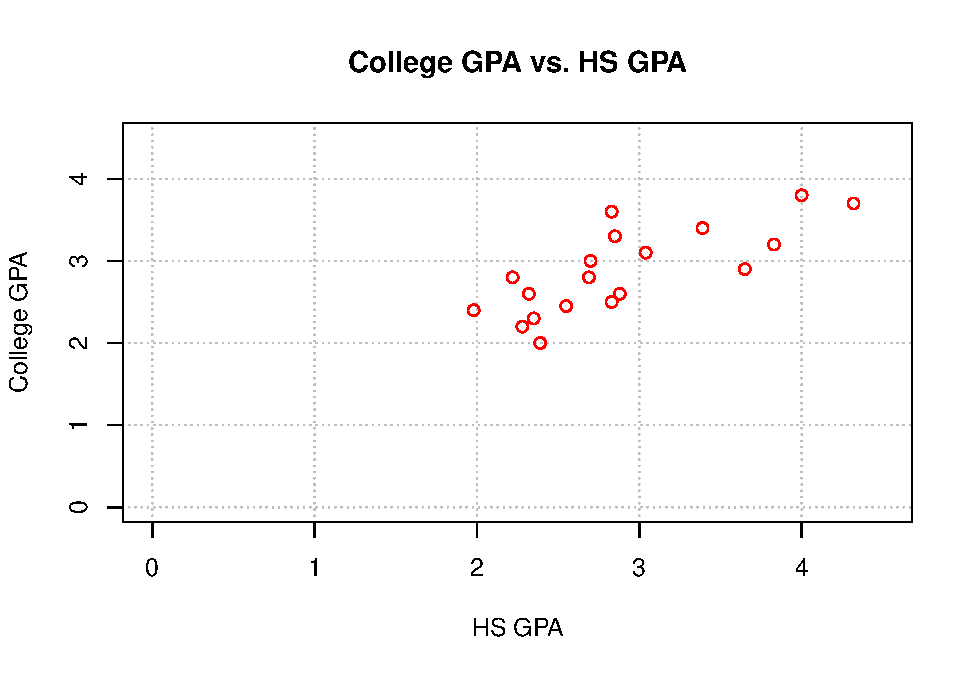
\includegraphics{01-Introduction-to-R_files/figure-latex/unnamed-chunk-27-1.pdf}
The \texttt{plot()} function creates a two dimensional plot of data.

Here are descriptions of its arguments:

\begin{itemize}
\item
  x specifies what is plotted for the x-axis.
\item
  y specifies what is plotted for the y-axis.
\item
  xlab and ylab specify the x-axis and y-axis labels, respectively.
\item
  main specifies the main title of the plot.
\item
  xlim and ylim specify the x-axis and y-axis limits, respectively.

  \begin{itemize}
  \tightlist
  \item
    Notice the use of the c() function.
  \end{itemize}
\item
  col specifies the color of the plotting points.

  \begin{itemize}
  \tightlist
  \item
    Run the \texttt{colors()} function to see what possible colors can be used.
  \item
    Also, you can see \href{https://github.com/EarlGlynn/colorchart/wiki/Color-Chart-in-R}{Here} for the colors from colors().
  \end{itemize}
\item
  \texttt{pch} specifies the plotting characters.
\item
  \texttt{cex}specifies the height of the plotting characters.
  The value 1.0 is the default.
\item
  \texttt{panel.first\ =\ grid()} specifies grid lines will be plotted.
\item
  The line types can be specified as follows:
  \texttt{1=solid,\ 2=dashed,\ 3=dotted,\ 4=dotdash,\ 5=longdash,\ 6=twodash} or as one of the character strings \texttt{"blank",\ "solid",\ "dashed",\ "dotted",\ \ "dotdash",\ "longdash"}, or \texttt{"twodash"}.\\
  These line type specifications can be used in other functions.\\
\item
  The \texttt{par()}(parameter) function's Help contains more information about the different plotting options!
\end{itemize}

\hypertarget{regression}{%
\section{Regression}\label{regression}}

Our model is:\[CollegeGPA=\beta_0+\beta_1HSGPA+\epsilon\]

\begin{Shaded}
\begin{Highlighting}[]
\NormalTok{mod.fit }\OtherTok{\textless{}{-}} \FunctionTok{lm}\NormalTok{(}\AttributeTok{formula=}\NormalTok{ CollegeGPA}\SpecialCharTok{\textasciitilde{}}\NormalTok{ HSGPA, }\AttributeTok{data=}\NormalTok{gpacsv)}
\NormalTok{mod.fit}
\CommentTok{\#\textgreater{} }
\CommentTok{\#\textgreater{} Call:}
\CommentTok{\#\textgreater{} lm(formula = CollegeGPA \textasciitilde{} HSGPA, data = gpacsv)}
\CommentTok{\#\textgreater{} }
\CommentTok{\#\textgreater{} Coefficients:}
\CommentTok{\#\textgreater{} (Intercept)        HSGPA  }
\CommentTok{\#\textgreater{}      1.0869       0.6125}
\end{Highlighting}
\end{Shaded}

\begin{Shaded}
\begin{Highlighting}[]
\FunctionTok{names}\NormalTok{(mod.fit)}
\CommentTok{\#\textgreater{}  [1] "coefficients"  "residuals"     "effects"      }
\CommentTok{\#\textgreater{}  [4] "rank"          "fitted.values" "assign"       }
\CommentTok{\#\textgreater{}  [7] "qr"            "df.residual"   "xlevels"      }
\CommentTok{\#\textgreater{} [10] "call"          "terms"         "model"}
\end{Highlighting}
\end{Shaded}

\begin{Shaded}
\begin{Highlighting}[]
\NormalTok{mod.fit}\SpecialCharTok{$}\NormalTok{coefficients}
\CommentTok{\#\textgreater{} (Intercept)       HSGPA }
\CommentTok{\#\textgreater{}   1.0868795   0.6124941}
\end{Highlighting}
\end{Shaded}

\begin{Shaded}
\begin{Highlighting}[]
\FunctionTok{round}\NormalTok{(mod.fit}\SpecialCharTok{$}\NormalTok{residuals[}\DecValTok{1}\SpecialCharTok{:}\DecValTok{5}\NormalTok{],}\DecValTok{2}\NormalTok{)}
\CommentTok{\#\textgreater{}     1     2     3     4     5 }
\CommentTok{\#\textgreater{}  0.15 {-}0.23  0.26 {-}0.20 {-}0.32}
\end{Highlighting}
\end{Shaded}

\begin{Shaded}
\begin{Highlighting}[]
\FunctionTok{library}\NormalTok{(tidyverse)}
\CommentTok{\#\textgreater{} {-}{-} Attaching packages {-}{-}{-}{-}{-}{-}{-}{-}{-}{-}{-}{-}{-}{-}{-}{-}{-}{-}{-} tidyverse 1.3.2 {-}{-}}
\CommentTok{\#\textgreater{} v ggplot2 3.4.1     v purrr   1.0.1}
\CommentTok{\#\textgreater{} v tibble  3.1.8     v dplyr   1.1.0}
\CommentTok{\#\textgreater{} v tidyr   1.3.0     v stringr 1.5.0}
\CommentTok{\#\textgreater{} v readr   2.1.4     v forcats 0.5.2}
\CommentTok{\#\textgreater{} {-}{-} Conflicts {-}{-}{-}{-}{-}{-}{-}{-}{-}{-}{-}{-}{-}{-}{-}{-}{-}{-}{-}{-}{-}{-} tidyverse\_conflicts() {-}{-}}
\CommentTok{\#\textgreater{} x dplyr::filter() masks stats::filter()}
\CommentTok{\#\textgreater{} x dplyr::lag()    masks stats::lag()}
\NormalTok{save.fit }\OtherTok{\textless{}{-}} \FunctionTok{data.frame}\NormalTok{(gpacsv, }\AttributeTok{C.GPA.hat =} 
    \FunctionTok{round}\NormalTok{(mod.fit}\SpecialCharTok{$}\NormalTok{fitted.values,}\DecValTok{2}\NormalTok{), }\AttributeTok{residuals =} 
    \FunctionTok{round}\NormalTok{(mod.fit}\SpecialCharTok{$}\NormalTok{residuals,}\DecValTok{2}\NormalTok{))}

\NormalTok{save.fit }\SpecialCharTok{\%\textgreater{}\%} \FunctionTok{head}\NormalTok{()}
\CommentTok{\#\textgreater{}   HSGPA CollegeGPA C.GPA.hat residuals}
\CommentTok{\#\textgreater{} 1  3.04       3.10      2.95      0.15}
\CommentTok{\#\textgreater{} 2  2.35       2.30      2.53     {-}0.23}
\CommentTok{\#\textgreater{} 3  2.70       3.00      2.74      0.26}
\CommentTok{\#\textgreater{} 4  2.55       2.45      2.65     {-}0.20}
\CommentTok{\#\textgreater{} 5  2.83       2.50      2.82     {-}0.32}
\CommentTok{\#\textgreater{} 6  4.32       3.70      3.73     {-}0.03}
\end{Highlighting}
\end{Shaded}

\begin{Shaded}
\begin{Highlighting}[]
\FunctionTok{summary}\NormalTok{(mod.fit)}
\CommentTok{\#\textgreater{} }
\CommentTok{\#\textgreater{} Call:}
\CommentTok{\#\textgreater{} lm(formula = CollegeGPA \textasciitilde{} HSGPA, data = gpacsv)}
\CommentTok{\#\textgreater{} }
\CommentTok{\#\textgreater{} Residuals:}
\CommentTok{\#\textgreater{}      Min       1Q   Median       3Q      Max }
\CommentTok{\#\textgreater{} {-}0.55074 {-}0.25086  0.01633  0.24242  0.77976 }
\CommentTok{\#\textgreater{} }
\CommentTok{\#\textgreater{} Coefficients:}
\CommentTok{\#\textgreater{}             Estimate Std. Error t value Pr(\textgreater{}|t|)    }
\CommentTok{\#\textgreater{} (Intercept)   1.0869     0.3666   2.965 0.008299 ** }
\CommentTok{\#\textgreater{} HSGPA         0.6125     0.1237   4.953 0.000103 ***}
\CommentTok{\#\textgreater{} {-}{-}{-}}
\CommentTok{\#\textgreater{} Signif. codes:  }
\CommentTok{\#\textgreater{} 0 \textquotesingle{}***\textquotesingle{} 0.001 \textquotesingle{}**\textquotesingle{} 0.01 \textquotesingle{}*\textquotesingle{} 0.05 \textquotesingle{}.\textquotesingle{} 0.1 \textquotesingle{} \textquotesingle{} 1}
\CommentTok{\#\textgreater{} }
\CommentTok{\#\textgreater{} Residual standard error: 0.3437 on 18 degrees of freedom}
\CommentTok{\#\textgreater{} Multiple R{-}squared:  0.5768, Adjusted R{-}squared:  0.5533 }
\CommentTok{\#\textgreater{} F{-}statistic: 24.54 on 1 and 18 DF,  p{-}value: 0.0001027}
\end{Highlighting}
\end{Shaded}

Hence, our estimated regression model is\[ \hat{collge.GPA}=\hat{\beta_0}+\hat{\beta_1}HS.GPA
=1.0869+0.6125HS.GPA\]

\begin{Shaded}
\begin{Highlighting}[]
\CommentTok{\# Open a new graphics window }
\CommentTok{\# device new}
\FunctionTok{dev.new}\NormalTok{(}\AttributeTok{width =} \DecValTok{8}\NormalTok{, }\AttributeTok{height =} \DecValTok{6}\NormalTok{, }\AttributeTok{pointsize =} \DecValTok{10}\NormalTok{)}


\CommentTok{\# 1 row and 2 columns of plots}
\FunctionTok{par}\NormalTok{(}\AttributeTok{mfrow =} \FunctionTok{c}\NormalTok{(}\DecValTok{1}\NormalTok{,}\DecValTok{2}\NormalTok{))}
\CommentTok{\# par= graphic parameter}
\CommentTok{\# mfrow= make a frame by row}

\CommentTok{\# Same scatter plot as before}
\FunctionTok{plot}\NormalTok{(}\AttributeTok{x =}\NormalTok{ gpacsv}\SpecialCharTok{$}\NormalTok{HSGPA, }\AttributeTok{y =}\NormalTok{ gpacsv}\SpecialCharTok{$}\NormalTok{CollegeGPA, }\AttributeTok{xlab =} \StringTok{"HS }
\StringTok{    GPA"}\NormalTok{, }\AttributeTok{ylab =} \StringTok{"College GPA"}\NormalTok{, }\AttributeTok{main =} \StringTok{"College GPA vs. }
\StringTok{    HS GPA"}\NormalTok{, }\AttributeTok{xlim =} \FunctionTok{c}\NormalTok{(}\DecValTok{0}\NormalTok{,}\FloatTok{4.5}\NormalTok{), }\AttributeTok{ylim =} \FunctionTok{c}\NormalTok{(}\DecValTok{0}\NormalTok{,}\FloatTok{4.5}\NormalTok{), }\AttributeTok{col =} 
    \StringTok{"red"}\NormalTok{, }\AttributeTok{pch =} \DecValTok{1}\NormalTok{, }\AttributeTok{cex =} \FloatTok{1.0}\NormalTok{, }\AttributeTok{panel.first =} \FunctionTok{grid}\NormalTok{(}\AttributeTok{col =} 
    \StringTok{"gray"}\NormalTok{, }\AttributeTok{lty =} \StringTok{"dotted"}\NormalTok{))}
    
\CommentTok{\# Puts the line y = a + bx on the plot}
\FunctionTok{abline}\NormalTok{(}\AttributeTok{a =}\NormalTok{ mod.fit}\SpecialCharTok{$}\NormalTok{coefficients[}\DecValTok{1}\NormalTok{], }\AttributeTok{b =} 
\NormalTok{    mod.fit}\SpecialCharTok{$}\NormalTok{coefficients[}\DecValTok{2}\NormalTok{], }\AttributeTok{lty =} \StringTok{"solid"}\NormalTok{, }\AttributeTok{col =} 
    \StringTok{"blue"}\NormalTok{, }\AttributeTok{lwd =} \DecValTok{2}\NormalTok{)}
    

\CommentTok{\# Same scatter plot as before}
\FunctionTok{plot}\NormalTok{(}\AttributeTok{x =}\NormalTok{ gpacsv}\SpecialCharTok{$}\NormalTok{HSGPA, }\AttributeTok{y =}\NormalTok{ gpacsv}\SpecialCharTok{$}\NormalTok{CollegeGPA, }\AttributeTok{xlab =} \StringTok{"HS }
\StringTok{    GPA"}\NormalTok{, }\AttributeTok{ylab =} \StringTok{"College GPA"}\NormalTok{, }\AttributeTok{main =} \StringTok{"College GPA vs. }
\StringTok{    HS GPA"}\NormalTok{, }\AttributeTok{xlim =} \FunctionTok{c}\NormalTok{(}\DecValTok{0}\NormalTok{,}\FloatTok{4.5}\NormalTok{), }\AttributeTok{ylim =} \FunctionTok{c}\NormalTok{(}\DecValTok{0}\NormalTok{,}\FloatTok{4.5}\NormalTok{), }\AttributeTok{col =} 
    \StringTok{"red"}\NormalTok{, }\AttributeTok{pch =} \DecValTok{1}\NormalTok{, }\AttributeTok{cex =} \FloatTok{1.0}\NormalTok{, }\AttributeTok{panel.first =} \FunctionTok{grid}\NormalTok{(}\AttributeTok{col =} 
    \StringTok{"gray"}\NormalTok{, }\AttributeTok{lty =} \StringTok{"dotted"}\NormalTok{))}


\CommentTok{\# Add line}
\CommentTok{\# expr= math expression}
\FunctionTok{curve}\NormalTok{(}\AttributeTok{expr =}\NormalTok{ mod.fit}\SpecialCharTok{$}\NormalTok{coefficients[}\DecValTok{1}\NormalTok{] }\SpecialCharTok{+} 
\NormalTok{    mod.fit}\SpecialCharTok{$}\NormalTok{coefficients[}\DecValTok{2}\NormalTok{]}\SpecialCharTok{*}\NormalTok{x, }
    \AttributeTok{xlim =} \FunctionTok{c}\NormalTok{(}\FunctionTok{min}\NormalTok{(gpacsv}\SpecialCharTok{$}\NormalTok{HSGPA),}\FunctionTok{max}\NormalTok{(gpacsv}\SpecialCharTok{$}\NormalTok{HSGPA)), }
    \AttributeTok{col=} \StringTok{"blue"}\NormalTok{, }\AttributeTok{add =} \ConstantTok{TRUE}\NormalTok{, }\AttributeTok{lwd =} \DecValTok{2}\NormalTok{)}
\end{Highlighting}
\end{Shaded}

\begin{itemize}
\item
  The \texttt{dev.new()} function can be used to open a new plotting window.
\item
  The \texttt{abline()} function can be used to draw straight lines on a plot. In the format used here, the line y = a + bx was drawn where a was the (intercept) and b was the (slope).
\item
  In the second plot, the curve() function was used to draw the line on the plot. This was done to have the line within the range of the high school GPA values.
\end{itemize}

Let's use function to automate what we have done.

\begin{Shaded}
\begin{Highlighting}[]
\NormalTok{my.reg.func }\OtherTok{\textless{}{-}} \ControlFlowTok{function}\NormalTok{(x, y, data) \{}

    \CommentTok{\# Fit the simple linear regression model and save the results in mod.fit}
\NormalTok{    mod.fit }\OtherTok{\textless{}{-}} \FunctionTok{lm}\NormalTok{(}\AttributeTok{formula =}\NormalTok{ y }\SpecialCharTok{\textasciitilde{}}\NormalTok{ x, }\AttributeTok{data =}\NormalTok{ data)}

    \CommentTok{\#Open a new graphics window {-} do not need to}
    \FunctionTok{dev.new}\NormalTok{(}\AttributeTok{width =} \DecValTok{6}\NormalTok{, }\AttributeTok{height =} \DecValTok{6}\NormalTok{, }\AttributeTok{pointsize =} \DecValTok{10}\NormalTok{)}

    \CommentTok{\# Same scatter plot as before}
    \FunctionTok{plot}\NormalTok{(}\AttributeTok{x =}\NormalTok{ x, }\AttributeTok{y =}\NormalTok{ y, }\AttributeTok{xlab =} \StringTok{"x"}\NormalTok{, }\AttributeTok{ylab =} \StringTok{"y"}\NormalTok{, }\AttributeTok{main =} \StringTok{"y vs. x"}\NormalTok{, }\AttributeTok{panel.first=}\FunctionTok{grid}\NormalTok{(}\AttributeTok{col =} \StringTok{"gray"}\NormalTok{, }\AttributeTok{lty =} 
      \StringTok{"dotted"}\NormalTok{))}

    \CommentTok{\# Plot model}
    \FunctionTok{curve}\NormalTok{(}\AttributeTok{expr =}\NormalTok{ mod.fit}\SpecialCharTok{$}\NormalTok{coefficients[}\DecValTok{1}\NormalTok{] }\SpecialCharTok{+} 
\NormalTok{      mod.fit}\SpecialCharTok{$}\NormalTok{coefficients[}\DecValTok{2}\NormalTok{]}\SpecialCharTok{*}\NormalTok{x, }\AttributeTok{xlim =} \FunctionTok{c}\NormalTok{(}\FunctionTok{min}\NormalTok{(x),}\FunctionTok{max}\NormalTok{(x)), }
      \AttributeTok{col =} \StringTok{"blue"}\NormalTok{, }\AttributeTok{add =} \ConstantTok{TRUE}\NormalTok{)}

    \CommentTok{\# This is the object returned}
\NormalTok{    mod.fit}
\NormalTok{  \}}
\end{Highlighting}
\end{Shaded}

\begin{Shaded}
\begin{Highlighting}[]
\NormalTok{save.it }\OtherTok{\textless{}{-}} \FunctionTok{my.reg.func}\NormalTok{(}\AttributeTok{x =}\NormalTok{ gpacsv}\SpecialCharTok{$}\NormalTok{HSGPA, }\AttributeTok{y =} 
\NormalTok{    gpacsv}\SpecialCharTok{$}\NormalTok{CollegeGPA, }\AttributeTok{data =}\NormalTok{ gpacsv)}
\end{Highlighting}
\end{Shaded}

To get specific x-axis or y-axis tick marks on a plot, use the \texttt{axis()} function. For example,

\begin{Shaded}
\begin{Highlighting}[]
\CommentTok{\#Note that xaxt = "n" tells R to not give any labels on the }
\CommentTok{\#  x{-}axis (yaxt = "n" works for y{-}axis)}
\FunctionTok{plot}\NormalTok{(}\AttributeTok{x =}\NormalTok{ gpacsv}\SpecialCharTok{$}\NormalTok{HSGPA, }\AttributeTok{y =}\NormalTok{ gpacsv}\SpecialCharTok{$}\NormalTok{CollegeGPA, }\AttributeTok{xlab =} \StringTok{"HS GPA"}\NormalTok{, }
     \AttributeTok{ylab =} \StringTok{"College GPA"}\NormalTok{, }\AttributeTok{main =} \StringTok{"College GPA vs. HS GPA"}\NormalTok{, }
     \AttributeTok{xaxt =} \StringTok{"n"}\NormalTok{, }\AttributeTok{xlim =} \FunctionTok{c}\NormalTok{(}\DecValTok{0}\NormalTok{, }\FloatTok{4.5}\NormalTok{), }\AttributeTok{ylim =} \FunctionTok{c}\NormalTok{(}\DecValTok{0}\NormalTok{, }\FloatTok{4.5}\NormalTok{), }\AttributeTok{col =} 
     \StringTok{"red"}\NormalTok{, }\AttributeTok{pch =} \DecValTok{1}\NormalTok{)}
\end{Highlighting}
\end{Shaded}

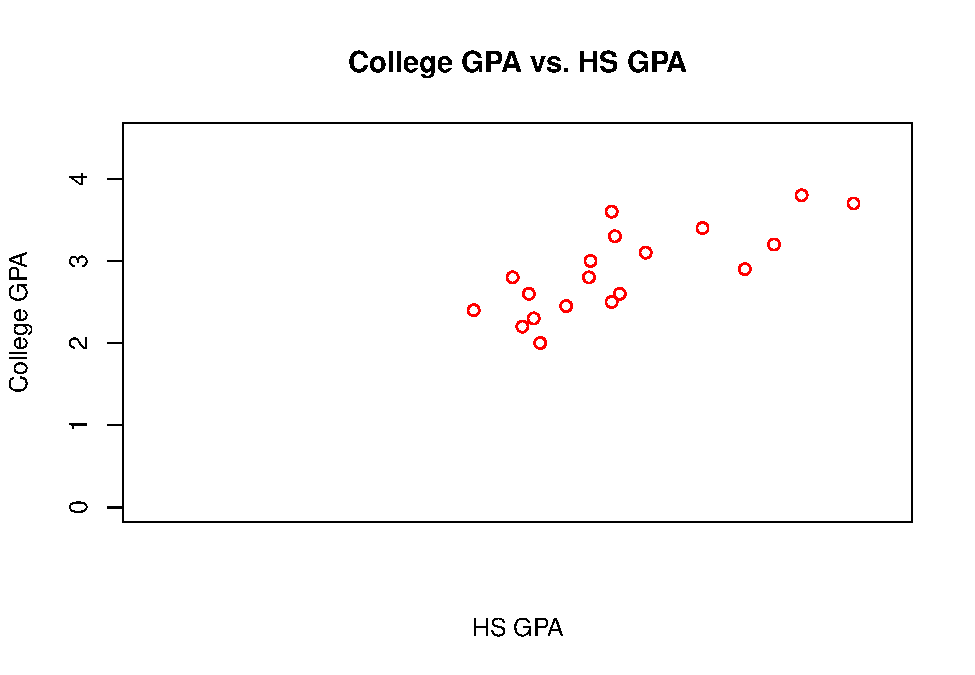
\includegraphics{01-Introduction-to-R_files/figure-latex/unnamed-chunk-37-1.pdf}

\begin{Shaded}
\begin{Highlighting}[]
\FunctionTok{plot}\NormalTok{(}\AttributeTok{x =}\NormalTok{ gpacsv}\SpecialCharTok{$}\NormalTok{HSGPA, }\AttributeTok{y =}\NormalTok{ gpacsv}\SpecialCharTok{$}\NormalTok{CollegeGPA, }\AttributeTok{xlab =} \StringTok{"HS GPA"}\NormalTok{, }
     \AttributeTok{ylab =} \StringTok{"College GPA"}\NormalTok{, }\AttributeTok{main =} \StringTok{"College GPA vs. HS GPA"}\NormalTok{, }
     \AttributeTok{xaxt =} \StringTok{"n"}\NormalTok{, }\AttributeTok{xlim =} \FunctionTok{c}\NormalTok{(}\DecValTok{0}\NormalTok{, }\FloatTok{4.5}\NormalTok{), }\AttributeTok{ylim =} \FunctionTok{c}\NormalTok{(}\DecValTok{0}\NormalTok{, }\FloatTok{4.5}\NormalTok{), }\AttributeTok{col =} 
     \StringTok{"red"}\NormalTok{, }\AttributeTok{pch =} \DecValTok{1}\NormalTok{)}
     
\CommentTok{\#Major tick marks}
\FunctionTok{axis}\NormalTok{(}\AttributeTok{side =} \DecValTok{1}\NormalTok{, }\AttributeTok{at =} \FunctionTok{seq}\NormalTok{(}\AttributeTok{from =} \DecValTok{0}\NormalTok{, }\AttributeTok{to =} \FloatTok{4.5}\NormalTok{, }\AttributeTok{by =} \FloatTok{0.5}\NormalTok{)) }
\end{Highlighting}
\end{Shaded}

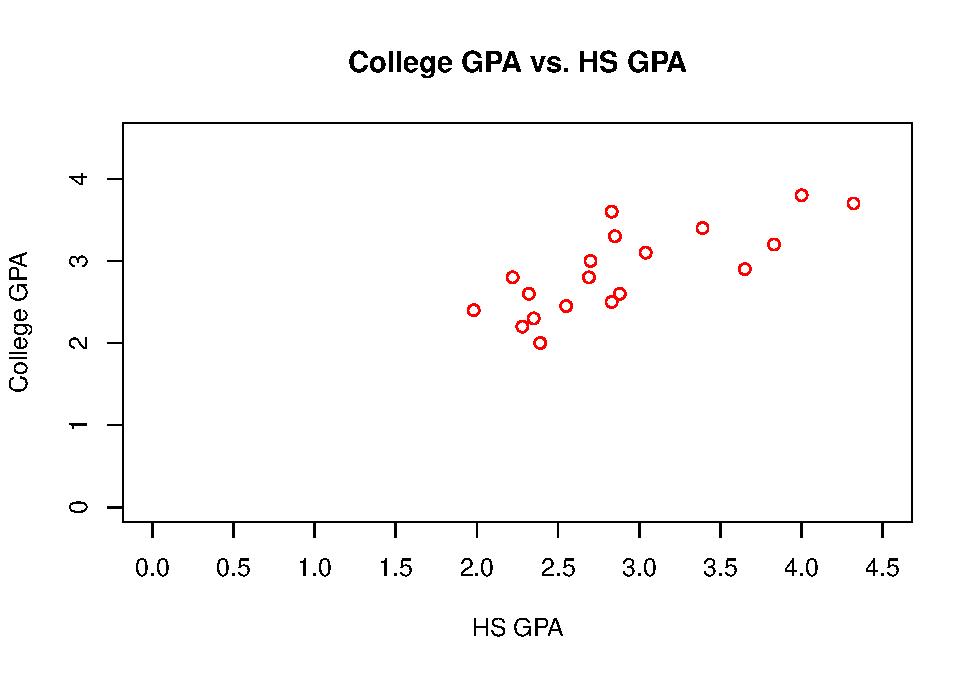
\includegraphics{01-Introduction-to-R_files/figure-latex/unnamed-chunk-38-1.pdf}

\begin{Shaded}
\begin{Highlighting}[]
\FunctionTok{plot}\NormalTok{(}\AttributeTok{x =}\NormalTok{ gpacsv}\SpecialCharTok{$}\NormalTok{HSGPA, }\AttributeTok{y =}\NormalTok{ gpacsv}\SpecialCharTok{$}\NormalTok{CollegeGPA, }\AttributeTok{xlab =} \StringTok{"HS GPA"}\NormalTok{, }
     \AttributeTok{ylab =} \StringTok{"College GPA"}\NormalTok{, }\AttributeTok{main =} \StringTok{"College GPA vs. HS GPA"}\NormalTok{, }
     \AttributeTok{xaxt =} \StringTok{"n"}\NormalTok{, }\AttributeTok{xlim =} \FunctionTok{c}\NormalTok{(}\DecValTok{0}\NormalTok{, }\FloatTok{4.5}\NormalTok{), }\AttributeTok{ylim =} \FunctionTok{c}\NormalTok{(}\DecValTok{0}\NormalTok{, }\FloatTok{4.5}\NormalTok{), }\AttributeTok{col =} 
     \StringTok{"red"}\NormalTok{, }\AttributeTok{pch =} \DecValTok{1}\NormalTok{)}
     
\CommentTok{\#Major tick marks}
\FunctionTok{axis}\NormalTok{(}\AttributeTok{side =} \DecValTok{1}\NormalTok{, }\AttributeTok{at =} \FunctionTok{seq}\NormalTok{(}\AttributeTok{from =} \DecValTok{0}\NormalTok{, }\AttributeTok{to =} \FloatTok{4.5}\NormalTok{, }\AttributeTok{by =} \FloatTok{0.5}\NormalTok{)) }

\CommentTok{\#Minor tick marks}
\FunctionTok{axis}\NormalTok{(}\AttributeTok{side =} \DecValTok{1}\NormalTok{, }\AttributeTok{at =} \FunctionTok{seq}\NormalTok{(}\AttributeTok{from =} \DecValTok{0}\NormalTok{, }\AttributeTok{to =} \FloatTok{4.5}\NormalTok{, }\AttributeTok{by =} \FloatTok{0.1}\NormalTok{), tck }
      \OtherTok{=} \FloatTok{0.01}\NormalTok{, }\AttributeTok{labels =} \ConstantTok{FALSE}\NormalTok{) }
\end{Highlighting}
\end{Shaded}

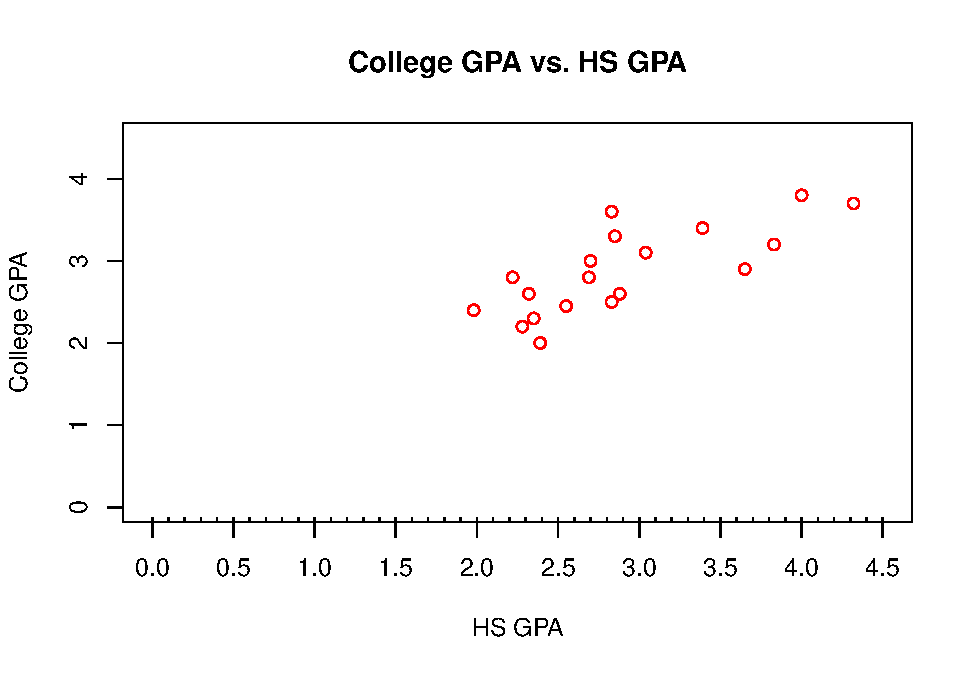
\includegraphics{01-Introduction-to-R_files/figure-latex/unnamed-chunk-39-1.pdf}

\hypertarget{object-oriented-language}{%
\section{Object-Oriented Language}\label{object-oriented-language}}

Functions are typically designed to operate on only one or very few classes of objects. However, some functions, like \texttt{summary()}, are \textbf{generic}, in the sense that essentially different versions of them have been constructed to work with different classes of objects.

When a generic function is run with an object, R first checks the object's class type and then looks to find a method function with the name format \texttt{\textless{}generic\ function\textgreater{}.\textless{}class\ name\textgreater{}}. Below are examples for \texttt{summary()}:

\begin{itemize}
\tightlist
\item
  summary(mod.fit) -- The function \texttt{summary.lm()} summarizes the regression model
\item
  summary(gpacsv) -- The function \texttt{summary.data.frame()} summarizes the data frame's contents
\item
  summary.default() -- R attempts to run this function if there is no method function for a class
\end{itemize}

There are many generic functions! For example, \texttt{plot()} is a generic function (try\texttt{plot(mod.fit)} to see what happens!). We will also see other generic functions like \texttt{predict()} later in the notes.

\begin{Shaded}
\begin{Highlighting}[]
\FunctionTok{plot}\NormalTok{(mod.fit)}
\end{Highlighting}
\end{Shaded}

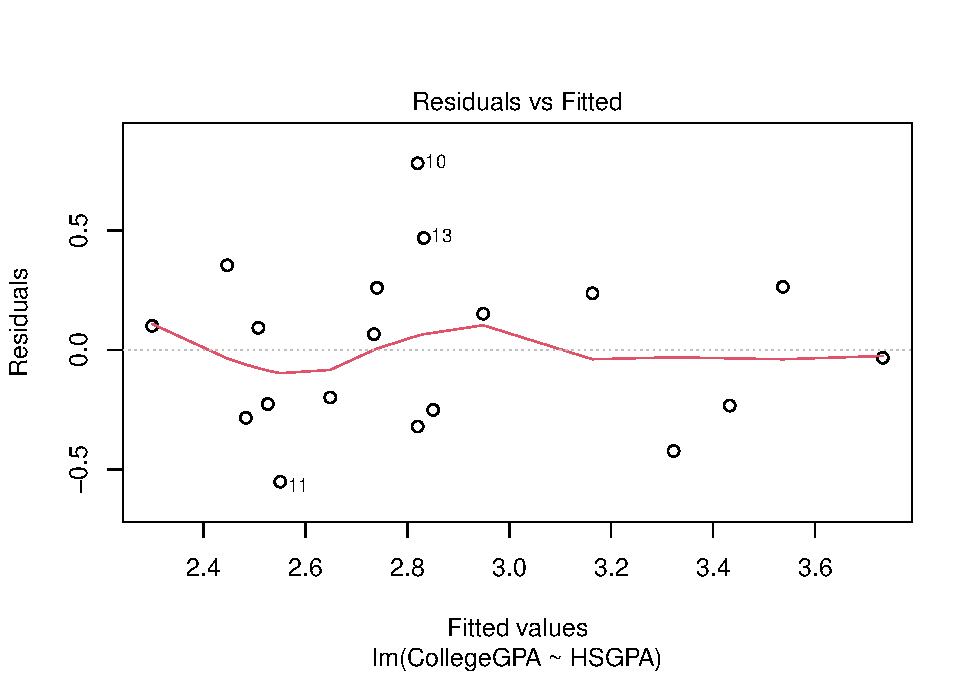
\includegraphics{01-Introduction-to-R_files/figure-latex/unnamed-chunk-40-1.pdf} 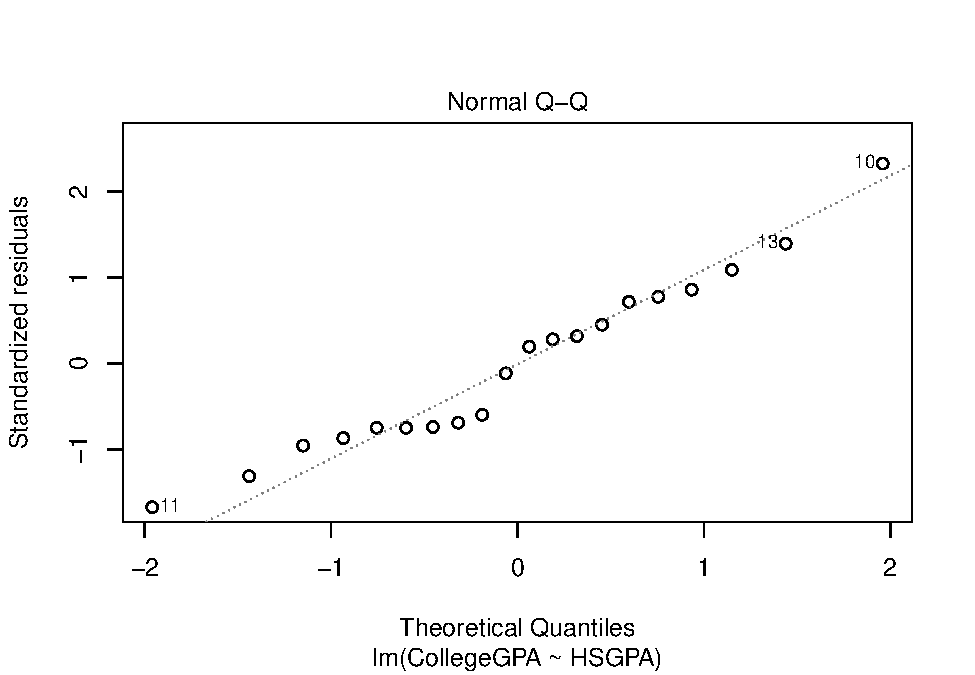
\includegraphics{01-Introduction-to-R_files/figure-latex/unnamed-chunk-40-2.pdf} 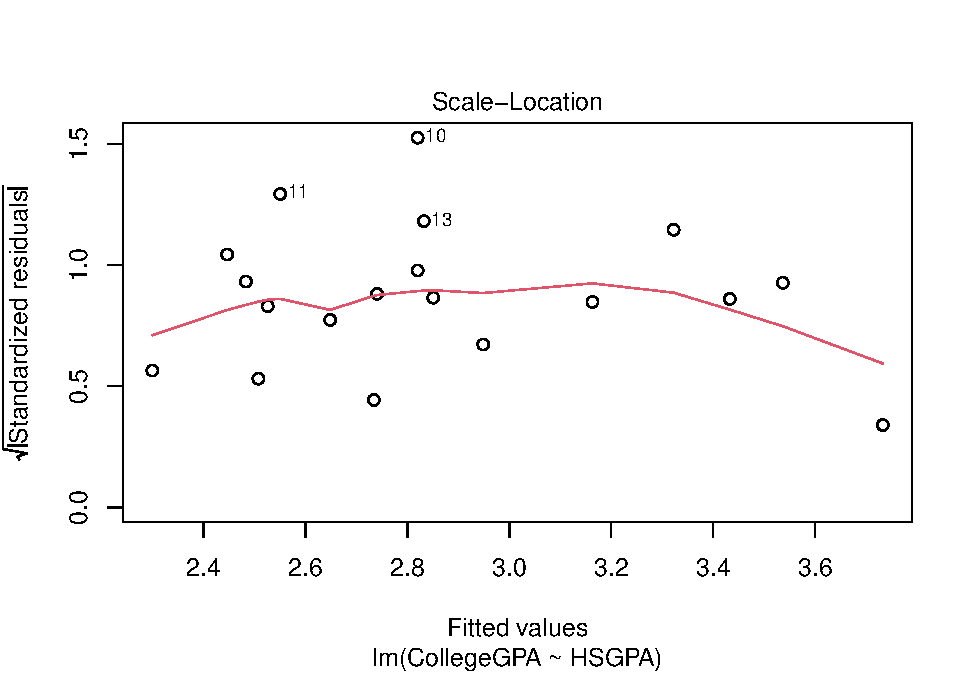
\includegraphics{01-Introduction-to-R_files/figure-latex/unnamed-chunk-40-3.pdf} 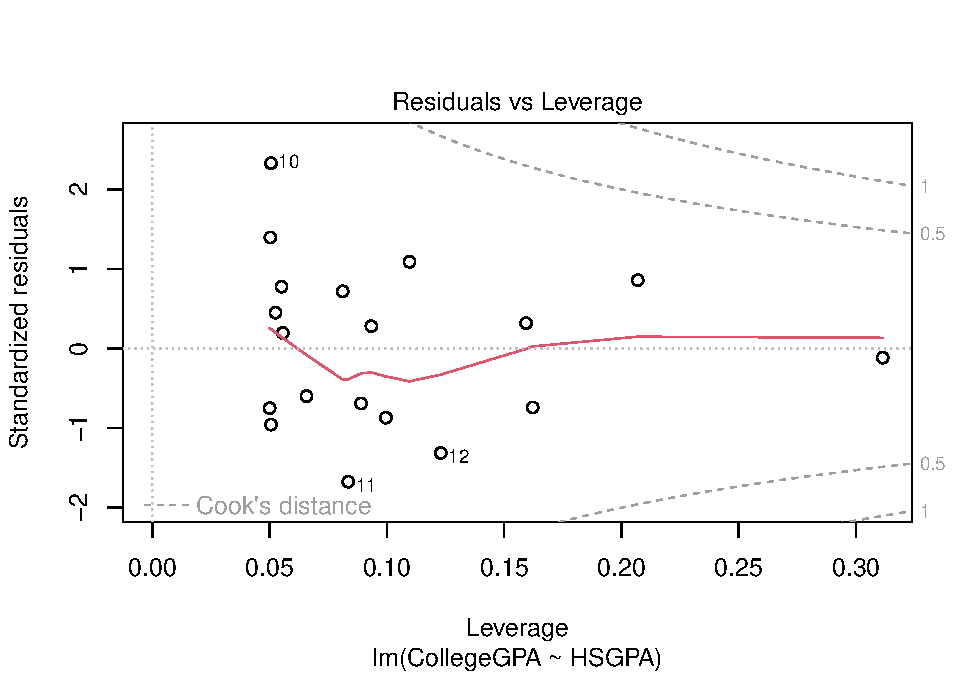
\includegraphics{01-Introduction-to-R_files/figure-latex/unnamed-chunk-40-4.pdf}

The purpose of generic functions is to use a familiar language set with any object. So it is convenient to use the same language set no matter the application. This is why R is referred to as an object-oriented language.

To see a list of all method functions associated with a class, use \texttt{methods(class\ =\ \textless{}class\ name\textgreater{})}. For the regression example, the method functions associated with the \texttt{lm} class are:

\begin{Shaded}
\begin{Highlighting}[]
\FunctionTok{methods}\NormalTok{(}\AttributeTok{class=}\StringTok{"lm"}\NormalTok{) }\SpecialCharTok{\%\textgreater{}\%} \FunctionTok{head}\NormalTok{()}
\CommentTok{\#\textgreater{} [1] "add1.lm"                   "alias.lm"                 }
\CommentTok{\#\textgreater{} [3] "anova.lm"                  "case.names.lm"            }
\CommentTok{\#\textgreater{} [5] "coerce,oldClass,S3{-}method" "confint.lm"}
\end{Highlighting}
\end{Shaded}

To see a list of all method functions for a generic function, use \texttt{methods(generic.function\ =\ \textless{}generic\ function\ name\textgreater{})}

\begin{Shaded}
\begin{Highlighting}[]
\FunctionTok{methods}\NormalTok{(}\AttributeTok{generic.function =} \StringTok{"summary"}\NormalTok{) }\SpecialCharTok{\%\textgreater{}\%} \FunctionTok{head}\NormalTok{()}
\CommentTok{\#\textgreater{} [1] "summary,ANY{-}method"           }
\CommentTok{\#\textgreater{} [2] "summary,DBIObject{-}method"     }
\CommentTok{\#\textgreater{} [3] "summary.aov"                  }
\CommentTok{\#\textgreater{} [4] "summary.aovlist"              }
\CommentTok{\#\textgreater{} [5] "summary.aspell"               }
\CommentTok{\#\textgreater{} [6] "summary.check\_packages\_in\_dir"}
\end{Highlighting}
\end{Shaded}

Knowing what a name of a particular method function can be helpful to find help on it. For example, the help for \texttt{summary()} alone is not very helpful! However, the help for \texttt{summary.lm()}provides a lot of useful information about what is summarized for a regression model.

\hypertarget{time-series-basics-plotting}{%
\chapter{Time Series Basics-Plotting}\label{time-series-basics-plotting}}

In this chapter, we will go over some \emph{Time Series} examples.
The aim of this chapter is to help you grasp some of the ideas about plotting.

\hypertarget{example-data}{%
\section{Example Data}\label{example-data}}

Click \href{http://www.chrisbilder.com/stat878/sections/2/OSU_enroll.csv}{OSU\_enroll.csv} to download data.

\begin{Shaded}
\begin{Highlighting}[]
\NormalTok{osu.enroll }\OtherTok{\textless{}{-}} \FunctionTok{read.csv}\NormalTok{(}\AttributeTok{file =} \StringTok{"OSU\_enroll.csv"}\NormalTok{, }
    \AttributeTok{stringsAsFactors =} \ConstantTok{TRUE}\NormalTok{)}
\end{Highlighting}
\end{Shaded}

\begin{Shaded}
\begin{Highlighting}[]
\FunctionTok{head}\NormalTok{(osu.enroll)}
\CommentTok{\#\textgreater{}   t Semester Year Enrollment      date}
\CommentTok{\#\textgreater{} 1 1     Fall 1989      20110 8/31/1989}
\CommentTok{\#\textgreater{} 2 2   Spring 1990      19128  2/1/1990}
\CommentTok{\#\textgreater{} 3 3   Summer 1990       7553  6/1/1990}
\CommentTok{\#\textgreater{} 4 4     Fall 1990      19591 8/31/1990}
\CommentTok{\#\textgreater{} 5 5   Spring 1991      18361  2/1/1991}
\CommentTok{\#\textgreater{} 6 6   Summer 1991       6702  6/1/1991}
\end{Highlighting}
\end{Shaded}

\begin{Shaded}
\begin{Highlighting}[]
\FunctionTok{tail}\NormalTok{(osu.enroll)}
\CommentTok{\#\textgreater{}     t Semester Year Enrollment      date}
\CommentTok{\#\textgreater{} 35 35   Spring 2001      20004  2/1/2001}
\CommentTok{\#\textgreater{} 36 36   Summer 2001       7558  6/1/2001}
\CommentTok{\#\textgreater{} 37 37     Fall 2001      21872 8/31/2001}
\CommentTok{\#\textgreater{} 38 38   Spring 2002      20922  2/1/2002}
\CommentTok{\#\textgreater{} 39 39   Summer 2002       7868  6/1/2002}
\CommentTok{\#\textgreater{} 40 40     Fall 2002      22992 8/31/2002}
\end{Highlighting}
\end{Shaded}

\begin{Shaded}
\begin{Highlighting}[]
\NormalTok{x }\OtherTok{\textless{}{-}}\NormalTok{ osu.enroll}\SpecialCharTok{$}\NormalTok{Enrollment}
\end{Highlighting}
\end{Shaded}

\begin{Shaded}
\begin{Highlighting}[]
\CommentTok{\#One way to do plot}
\FunctionTok{dev.new}\NormalTok{(}\AttributeTok{width =} \DecValTok{8}\NormalTok{, }\AttributeTok{height =} \DecValTok{6}\NormalTok{, }\AttributeTok{pointsize =} \DecValTok{10}\NormalTok{) }

\CommentTok{\# we did not specify y{-}axis and R put our x in y{-}axis, time in  x{-}axis}

\FunctionTok{plot}\NormalTok{(}\AttributeTok{x =}\NormalTok{ x, }\AttributeTok{ylab =} \StringTok{"OSU Enrollment"}\NormalTok{, }
       \AttributeTok{xlab =} \StringTok{"t (time)"}\NormalTok{, }\AttributeTok{type=}\StringTok{"l"}\NormalTok{, }\AttributeTok{col =} \StringTok{"red"}\NormalTok{, }
       \AttributeTok{main =} \StringTok{"OSU Enrollment from Fall 1989 to Fall 2002"}\NormalTok{, }
       \AttributeTok{panel.first =} \FunctionTok{grid}\NormalTok{(}\AttributeTok{col =} \StringTok{"gray"}\NormalTok{, }\AttributeTok{lty =} \StringTok{"dotted"}\NormalTok{))}
\end{Highlighting}
\end{Shaded}

\begin{Shaded}
\begin{Highlighting}[]
\FunctionTok{dev.new}\NormalTok{(}\AttributeTok{width =} \DecValTok{8}\NormalTok{, }\AttributeTok{height =} \DecValTok{6}\NormalTok{, }\AttributeTok{pointsize =} \DecValTok{10}\NormalTok{) }

\CommentTok{\# we did not specify y{-}axis and R put our x in y{-}axis, time in  x{-}axis}

\FunctionTok{plot}\NormalTok{(}\AttributeTok{x =}\NormalTok{ x, }\AttributeTok{ylab =} \StringTok{"OSU Enrollment"}\NormalTok{, }
       \AttributeTok{xlab =} \StringTok{"t (time)"}\NormalTok{, }\AttributeTok{type=}\StringTok{"l"}\NormalTok{, }\AttributeTok{col =} \StringTok{"red"}\NormalTok{, }
       \AttributeTok{main =} \StringTok{"OSU Enrollment from Fall 1989 to Fall 2002"}\NormalTok{, }
       \AttributeTok{panel.first =} \FunctionTok{grid}\NormalTok{(}\AttributeTok{col =} \StringTok{"gray"}\NormalTok{, }\AttributeTok{lty =} \StringTok{"dotted"}\NormalTok{))}

\FunctionTok{points}\NormalTok{(}\AttributeTok{x =}\NormalTok{ osu.enroll}\SpecialCharTok{$}\NormalTok{Enrollment, }\AttributeTok{pch =} \DecValTok{20}\NormalTok{, }\AttributeTok{col =} \StringTok{"blue"}\NormalTok{)}
\end{Highlighting}
\end{Shaded}

Altenatively, you can do the same thing using ggplot.

\begin{Shaded}
\begin{Highlighting}[]
\FunctionTok{library}\NormalTok{(ggplot2)}

\CommentTok{\# Create a data frame}
\NormalTok{df }\OtherTok{\textless{}{-}} \FunctionTok{data.frame}\NormalTok{(osu.enroll)}

\CommentTok{\# Create the plot}
\FunctionTok{ggplot}\NormalTok{(df, }\FunctionTok{aes}\NormalTok{(}\AttributeTok{x =}\NormalTok{ t, }\AttributeTok{y =}\NormalTok{ Enrollment)) }\SpecialCharTok{+}
  \FunctionTok{geom\_line}\NormalTok{(}\AttributeTok{colour =} \StringTok{"red"}\NormalTok{) }\SpecialCharTok{+}  \CommentTok{\# Line plot}
  \FunctionTok{geom\_point}\NormalTok{(}\AttributeTok{shape =} \DecValTok{20}\NormalTok{, }\AttributeTok{colour =} \StringTok{"blue"}\NormalTok{) }\SpecialCharTok{+}  \CommentTok{\# Add points}
  \FunctionTok{labs}\NormalTok{(}\AttributeTok{x =} \StringTok{"t (time)"}\NormalTok{, }\AttributeTok{y =} \StringTok{"OSU Enrollment"}\NormalTok{, }
       \AttributeTok{title =} \StringTok{"OSU Enrollment from Fall 1989 to Fall 2002"}\NormalTok{) }\SpecialCharTok{+}  \CommentTok{\# Set axis labels and title}
  \FunctionTok{theme\_bw}\NormalTok{() }\SpecialCharTok{+}  \CommentTok{\# Set the theme to a white background with black lines}
  \FunctionTok{theme}\NormalTok{(}\AttributeTok{panel.grid.major =} \FunctionTok{element\_line}\NormalTok{(}\AttributeTok{colour =} \StringTok{"gray"}\NormalTok{, }\AttributeTok{linetype =} \StringTok{"dotted"}\NormalTok{))  }\CommentTok{\# Add gray dotted lines to the plot}
\end{Highlighting}
\end{Shaded}

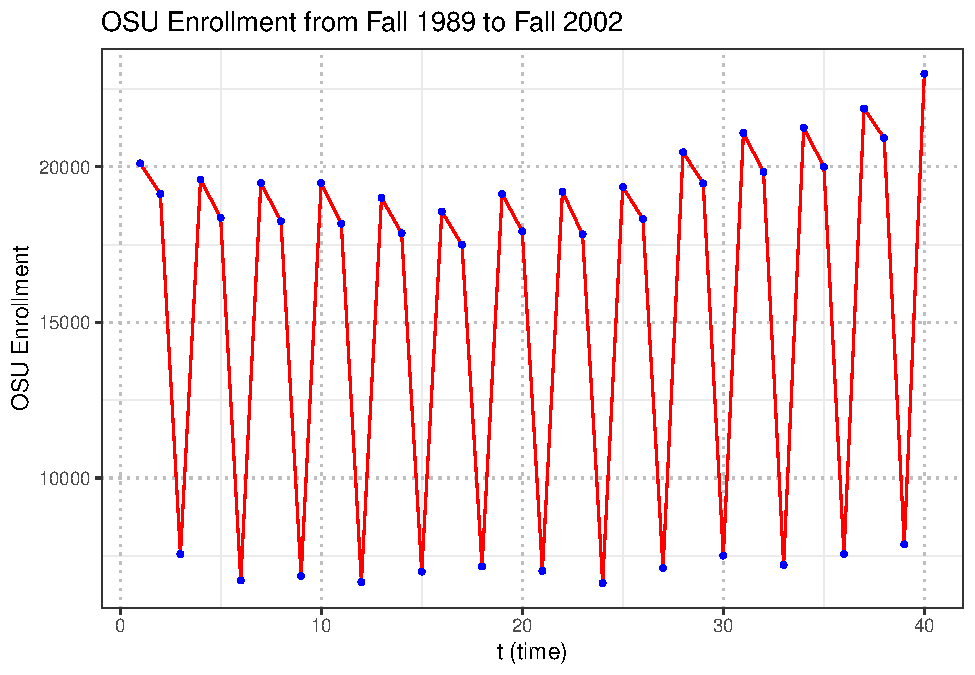
\includegraphics{02-Time-Series-Basics_files/figure-latex/unnamed-chunk-7-1.pdf}

When only x is specified in the \texttt{plot()} function, R puts this on the y-axis and uses the observation number on the x-axis.

Compare this to the next plot below where both x and y arguments are specified.

\begin{Shaded}
\begin{Highlighting}[]
\CommentTok{\#More complicated plot}
\NormalTok{fall }\OtherTok{\textless{}{-}}\NormalTok{ osu.enroll[osu.enroll}\SpecialCharTok{$}\NormalTok{Semester }\SpecialCharTok{==} \StringTok{"Fall"}\NormalTok{,]}
\NormalTok{spring }\OtherTok{\textless{}{-}}\NormalTok{ osu.enroll[osu.enroll}\SpecialCharTok{$}\NormalTok{Semester }\SpecialCharTok{==} \StringTok{"Spring"}\NormalTok{,]}
\NormalTok{summer }\OtherTok{\textless{}{-}}\NormalTok{ osu.enroll[osu.enroll}\SpecialCharTok{$}\NormalTok{Semester }\SpecialCharTok{==} \StringTok{"Summer"}\NormalTok{,]}

\FunctionTok{plot}\NormalTok{(}\AttributeTok{y =}\NormalTok{ fall}\SpecialCharTok{$}\NormalTok{Enrollment, }\AttributeTok{x =}\NormalTok{ fall}\SpecialCharTok{$}\NormalTok{t,}
    \AttributeTok{ylab =} \StringTok{"OSU Enrollment"}\NormalTok{, }\AttributeTok{xlab =} \StringTok{"t (time)"}\NormalTok{, }
    \AttributeTok{col =} \StringTok{"blue"}\NormalTok{, }
    \AttributeTok{main =} \StringTok{"OSU Enrollment from Fall 1989 to Fall 2002"}\NormalTok{, }
    \AttributeTok{panel.first =} \FunctionTok{grid}\NormalTok{(}\AttributeTok{col =} \StringTok{"gray"}\NormalTok{, }\AttributeTok{lty =} \StringTok{"dotted"}\NormalTok{), }
    \AttributeTok{pch =} \DecValTok{1}\NormalTok{, }\AttributeTok{type =} \StringTok{"o"}\NormalTok{, }\AttributeTok{ylim =} \FunctionTok{c}\NormalTok{(}\DecValTok{0}\NormalTok{,}\FunctionTok{max}\NormalTok{(osu.enroll}\SpecialCharTok{$}\NormalTok{Enrollment)))}

\FunctionTok{lines}\NormalTok{(}\AttributeTok{y =}\NormalTok{ spring}\SpecialCharTok{$}\NormalTok{Enrollment, }\AttributeTok{x =}\NormalTok{ spring}\SpecialCharTok{$}\NormalTok{t, }\AttributeTok{col =} \StringTok{"red"}\NormalTok{, }
    \AttributeTok{type =} \StringTok{"o"}\NormalTok{, }\AttributeTok{pch =} \DecValTok{2}\NormalTok{)}

\FunctionTok{lines}\NormalTok{(}\AttributeTok{y =}\NormalTok{ summer}\SpecialCharTok{$}\NormalTok{Enrollment, }\AttributeTok{x =}\NormalTok{ summer}\SpecialCharTok{$}\NormalTok{t, }\AttributeTok{col =} 
    \StringTok{"darkgreen"}\NormalTok{, }\AttributeTok{type =} \StringTok{"o"}\NormalTok{, }\AttributeTok{pch =} \DecValTok{3}\NormalTok{)}
    
\FunctionTok{legend}\NormalTok{(}\AttributeTok{x=}\StringTok{"center"}\NormalTok{, }\AttributeTok{legend=} \FunctionTok{c}\NormalTok{(}\StringTok{"Fall"}\NormalTok{,}\StringTok{"Spring"}\NormalTok{,}\StringTok{"Summer"}\NormalTok{), }\AttributeTok{pch=}\FunctionTok{c}\NormalTok{(}\DecValTok{1}\NormalTok{,}\DecValTok{2}\NormalTok{,}\DecValTok{3}\NormalTok{), }\AttributeTok{lty=}\FunctionTok{c}\NormalTok{(}\DecValTok{1}\NormalTok{,}\DecValTok{1}\NormalTok{,}\DecValTok{1}\NormalTok{), }\AttributeTok{col=}\FunctionTok{c}\NormalTok{(}\StringTok{"blue"}\NormalTok{,}\StringTok{"red"}\NormalTok{,}\StringTok{"darkgreen"}\NormalTok{), }\AttributeTok{bty=}\StringTok{"n"}\NormalTok{)}
\end{Highlighting}
\end{Shaded}

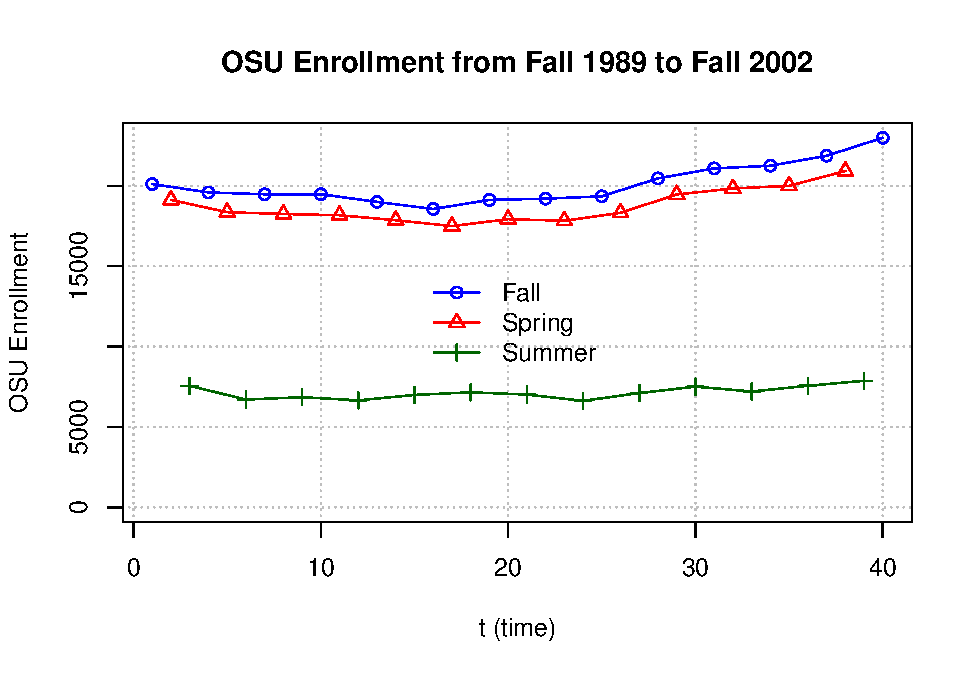
\includegraphics{02-Time-Series-Basics_files/figure-latex/unnamed-chunk-8-1.pdf}

\begin{Shaded}
\begin{Highlighting}[]
\CommentTok{\#Another way to do plot with actual dates}
\FunctionTok{plot}\NormalTok{(}\AttributeTok{y =}\NormalTok{ osu.enroll}\SpecialCharTok{$}\NormalTok{Enrollment, }
    \AttributeTok{x =} \FunctionTok{as.Date}\NormalTok{(osu.enroll}\SpecialCharTok{$}\NormalTok{date, }\AttributeTok{format =} \StringTok{"\%m/\%d/\%Y"}\NormalTok{), }
    \AttributeTok{xlab =} \StringTok{"Time"}\NormalTok{, }\AttributeTok{type =} \StringTok{"l"}\NormalTok{, }\AttributeTok{col =} \StringTok{"red"}\NormalTok{,  }
    \AttributeTok{main =} \StringTok{"OSU Enrollment from Fall 1989 to Fall 2002"}\NormalTok{,}
    \AttributeTok{ylab =} \StringTok{"OSU Enrollment"}\NormalTok{)}

\FunctionTok{points}\NormalTok{(}\AttributeTok{y =}\NormalTok{ osu.enroll}\SpecialCharTok{$}\NormalTok{Enrollment, }
    \AttributeTok{x =} \FunctionTok{as.Date}\NormalTok{(osu.enroll}\SpecialCharTok{$}\NormalTok{date, }\AttributeTok{format =} \StringTok{"\%m/\%d/\%Y"}\NormalTok{), pch }
    \OtherTok{=} \DecValTok{20}\NormalTok{, }\AttributeTok{col =} \StringTok{"blue"}\NormalTok{)}

\CommentTok{\#Create own gridlines}
\CommentTok{\# v specifies vertical line; h specifies horizontal line}
 \FunctionTok{abline}\NormalTok{(}\AttributeTok{v =} \FunctionTok{as.Date}\NormalTok{(}\FunctionTok{c}\NormalTok{(}\StringTok{"1990/1/1"}\NormalTok{, }\StringTok{"1992/1/1"}\NormalTok{, }\StringTok{"1994/1/1"}\NormalTok{, }
    \StringTok{"1996/1/1"}\NormalTok{, }\StringTok{"1998/1/1"}\NormalTok{, }\StringTok{"2000/1/1"}\NormalTok{, }\StringTok{"2002/1/1"}\NormalTok{)),}
    \AttributeTok{lty =} \StringTok{"dotted"}\NormalTok{, }\AttributeTok{col =} \StringTok{"lightgray"}\NormalTok{)}
 \FunctionTok{abline}\NormalTok{(}\AttributeTok{h =} \FunctionTok{c}\NormalTok{(}\DecValTok{10000}\NormalTok{, }\DecValTok{15000}\NormalTok{, }\DecValTok{20000}\NormalTok{), }\AttributeTok{lty =} \StringTok{"dotted"}\NormalTok{, }\AttributeTok{col =} 
    \StringTok{"lightgray"}\NormalTok{)}
\end{Highlighting}
\end{Shaded}

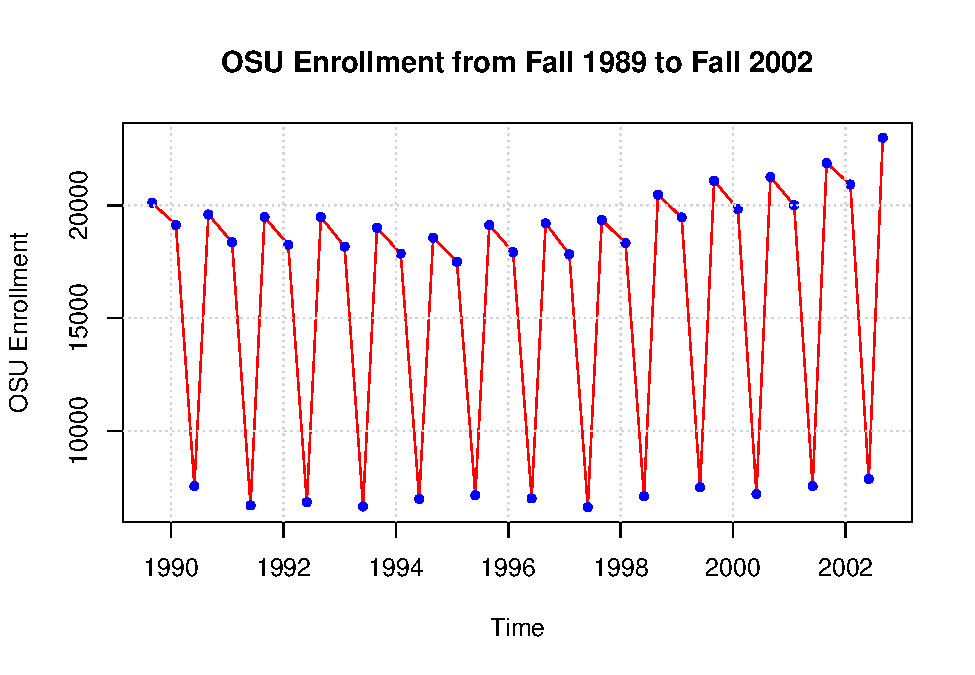
\includegraphics{02-Time-Series-Basics_files/figure-latex/unnamed-chunk-9-1.pdf}

\hypertarget{sp500-index}{%
\section{S\&P500 Index}\label{sp500-index}}

Click \href{http://www.chrisbilder.com/stat878/sections/2/SP500weekly.csv}{SP500weekly.csv} to download data.

\begin{Shaded}
\begin{Highlighting}[]
\NormalTok{SP500 }\OtherTok{\textless{}{-}} \FunctionTok{read.csv}\NormalTok{(}\AttributeTok{file=}\StringTok{"SP500weekly.csv"}\NormalTok{,}\AttributeTok{stringsAsFactors =} \ConstantTok{TRUE}\NormalTok{)}
\end{Highlighting}
\end{Shaded}

\begin{Shaded}
\begin{Highlighting}[]
\FunctionTok{head}\NormalTok{(SP500)}
\CommentTok{\#\textgreater{}   WeekStart   Open   High    Low  Close AdjClose     Volume}
\CommentTok{\#\textgreater{} 1  1/1/1995 459.21 462.49 457.20 460.68   460.68 1199080000}
\CommentTok{\#\textgreater{} 2  1/8/1995 460.67 466.43 458.65 465.97   465.97 1627330000}
\CommentTok{\#\textgreater{} 3 1/15/1995 465.97 470.43 463.99 464.78   464.78 1667400000}
\CommentTok{\#\textgreater{} 4 1/22/1995 464.78 471.36 461.14 470.39   470.39 1628110000}
\CommentTok{\#\textgreater{} 5 1/29/1995 470.39 479.91 467.49 478.65   478.65 1888560000}
\CommentTok{\#\textgreater{} 6  2/5/1995 478.64 482.60 478.36 481.46   481.46 1579920000}
\end{Highlighting}
\end{Shaded}

\begin{Shaded}
\begin{Highlighting}[]
\FunctionTok{tail}\NormalTok{(SP500)}
\CommentTok{\#\textgreater{}       WeekStart    Open    High     Low   Close AdjClose}
\CommentTok{\#\textgreater{} 1395  9/19/2021 4402.95 4465.40 4305.91 4455.48  4455.48}
\CommentTok{\#\textgreater{} 1396  9/26/2021 4442.12 4457.30 4288.52 4357.04  4357.04}
\CommentTok{\#\textgreater{} 1397  10/3/2021 4348.84 4429.97 4278.94 4391.34  4391.34}
\CommentTok{\#\textgreater{} 1398 10/10/2021 4385.44 4475.82 4329.92 4471.37  4471.37}
\CommentTok{\#\textgreater{} 1399 10/17/2021 4463.72 4559.67 4447.47 4544.90  4544.90}
\CommentTok{\#\textgreater{} 1400 10/24/2021 4553.69 4608.08 4537.36 4605.38  4605.38}
\CommentTok{\#\textgreater{}           Volume}
\CommentTok{\#\textgreater{} 1395 15697030000}
\CommentTok{\#\textgreater{} 1396 15555390000}
\CommentTok{\#\textgreater{} 1397 14795520000}
\CommentTok{\#\textgreater{} 1398 13758090000}
\CommentTok{\#\textgreater{} 1399 13966070000}
\CommentTok{\#\textgreater{} 1400 16206040000}
\end{Highlighting}
\end{Shaded}

\begin{Shaded}
\begin{Highlighting}[]
\NormalTok{x }\OtherTok{\textless{}{-}}\NormalTok{ SP500}\SpecialCharTok{$}\NormalTok{Close}
\end{Highlighting}
\end{Shaded}

\begin{Shaded}
\begin{Highlighting}[]
\CommentTok{\#One way to do plot}
\FunctionTok{dev.new}\NormalTok{(}\AttributeTok{width =} \DecValTok{8}\NormalTok{, }\AttributeTok{height =} \DecValTok{6}\NormalTok{, }\AttributeTok{pointsize =} \DecValTok{10}\NormalTok{) }
\CommentTok{\#again, we do not specify y{-}axis here}
\FunctionTok{plot}\NormalTok{(}\AttributeTok{x =}\NormalTok{ x, }\AttributeTok{ylab =} \StringTok{"S\&P 500 Index"}\NormalTok{, }\AttributeTok{xlab =} \StringTok{"t (time)"}\NormalTok{, }
    \AttributeTok{type =} \StringTok{"l"}\NormalTok{, }\AttributeTok{col =} \StringTok{"red"}\NormalTok{, }\AttributeTok{main =} \StringTok{"S\&P 500 Index from }
\StringTok{    1/1/1995 to 10/25/2021 (weekly)"}\NormalTok{, }
    \AttributeTok{panel.first =} \FunctionTok{grid}\NormalTok{(}\AttributeTok{col =} \StringTok{"gray"}\NormalTok{, }\AttributeTok{lty =} \StringTok{"dotted"}\NormalTok{))}
\end{Highlighting}
\end{Shaded}

\begin{Shaded}
\begin{Highlighting}[]
\CommentTok{\#Another way to do plot with actual dates}
\FunctionTok{plot}\NormalTok{(}\AttributeTok{y =}\NormalTok{ x, }\AttributeTok{x =} \FunctionTok{as.Date}\NormalTok{(SP500}\SpecialCharTok{$}\NormalTok{WeekStart, }\AttributeTok{format =}
    \StringTok{"\%m/\%d/\%Y"}\NormalTok{), }\AttributeTok{xlab =} \StringTok{"Time"}\NormalTok{, }\AttributeTok{type =} \StringTok{"l"}\NormalTok{, }\AttributeTok{col =} \StringTok{"red"}\NormalTok{, main }
    \OtherTok{=} \StringTok{"S\&P 500 Index from 1/1/1995 to 10/25/2021 (weekly)"}\NormalTok{,}
    \AttributeTok{ylab =} \StringTok{"S\&P 500 Index"}\NormalTok{)}

\CommentTok{\#Create own gridlines}
\FunctionTok{abline}\NormalTok{(}\AttributeTok{v =} \FunctionTok{as.Date}\NormalTok{(}\FunctionTok{c}\NormalTok{(}\StringTok{"1995/1/1"}\NormalTok{, }\StringTok{"2000/1/1"}\NormalTok{, }\StringTok{"2005/1/1"}\NormalTok{, }
    \StringTok{"2010/1/1"}\NormalTok{, }\StringTok{"2015/1/1"}\NormalTok{, }\StringTok{"2020/1/1"}\NormalTok{)), }\AttributeTok{lty =} \StringTok{"dotted"}\NormalTok{, }
    \AttributeTok{col =} \StringTok{"lightgray"}\NormalTok{)}

\FunctionTok{abline}\NormalTok{(}\AttributeTok{h =} \FunctionTok{seq}\NormalTok{(}\AttributeTok{from =} \DecValTok{0}\NormalTok{, }\AttributeTok{to =} \DecValTok{5000}\NormalTok{, }\AttributeTok{by =} \DecValTok{1000}\NormalTok{), }\AttributeTok{lty =} 
    \StringTok{"dotted"}\NormalTok{, }\AttributeTok{col =} \StringTok{"lightgray"}\NormalTok{)}
\end{Highlighting}
\end{Shaded}

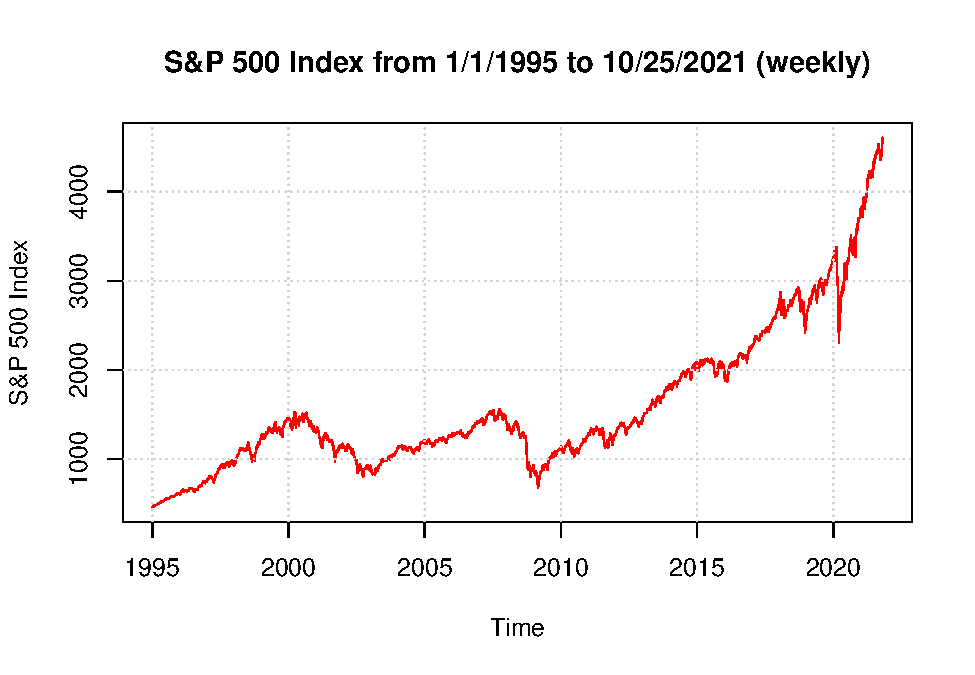
\includegraphics{02-Time-Series-Basics_files/figure-latex/unnamed-chunk-15-1.pdf}

\begin{Shaded}
\begin{Highlighting}[]
\CommentTok{\# One more way with fine control of the dates}
\FunctionTok{plot}\NormalTok{(}\AttributeTok{y =}\NormalTok{ x, }\AttributeTok{x =} \FunctionTok{as.Date}\NormalTok{(SP500}\SpecialCharTok{$}\NormalTok{WeekStart, }\AttributeTok{format =} 
    \StringTok{"\%m/\%d/\%Y"}\NormalTok{), }\AttributeTok{xlab =} \StringTok{"Time"}\NormalTok{, }\AttributeTok{type =} \StringTok{"l"}\NormalTok{, }\AttributeTok{col =} \StringTok{"red"}\NormalTok{, }
    \AttributeTok{main =} \StringTok{"S\&P 500 Index from 1/1/1995 to 10/25/2021 }
\StringTok{    (weekly)"}\NormalTok{, }\AttributeTok{ylab =} \StringTok{"S\&P 500 Index"}\NormalTok{, }\AttributeTok{xaxt =} \StringTok{"n"}\NormalTok{)}

\FunctionTok{axis.Date}\NormalTok{(}\AttributeTok{side =} \DecValTok{1}\NormalTok{, }\AttributeTok{at =} \FunctionTok{seq}\NormalTok{(}\AttributeTok{from =} \FunctionTok{as.Date}\NormalTok{(}\StringTok{"1995/1/1"}\NormalTok{),}
    \AttributeTok{to =} \FunctionTok{as.Date}\NormalTok{(}\StringTok{"2021/12/31"}\NormalTok{), }\AttributeTok{by =} \StringTok{"years"}\NormalTok{), }\AttributeTok{labels =} 
    \FunctionTok{format}\NormalTok{(}\AttributeTok{x =} \FunctionTok{seq}\NormalTok{(}\AttributeTok{from =} \FunctionTok{as.Date}\NormalTok{(}\StringTok{"1995/1/1"}\NormalTok{), }\AttributeTok{to =} 
    \FunctionTok{as.Date}\NormalTok{(}\StringTok{"2021/12/31"}\NormalTok{), }\AttributeTok{by =} \StringTok{"years"}\NormalTok{), }\AttributeTok{format =} \StringTok{"\%b\%y"}\NormalTok{), }
    \AttributeTok{las =} \DecValTok{2}\NormalTok{)  }\CommentTok{\#las changes orientation of labels}

\CommentTok{\#Create own gridlines}
\FunctionTok{abline}\NormalTok{(}\AttributeTok{v =} \FunctionTok{as.Date}\NormalTok{(}\FunctionTok{c}\NormalTok{(}\StringTok{"1995/1/1"}\NormalTok{, }\StringTok{"2000/1/1"}\NormalTok{, }\StringTok{"2005/1/1"}\NormalTok{, }
    \StringTok{"2010/1/1"}\NormalTok{, }\StringTok{"2015/1/1"}\NormalTok{, }\StringTok{"2020/1/1"}\NormalTok{)), }\AttributeTok{lty =} \StringTok{"dotted"}\NormalTok{, }
    \AttributeTok{col =} \StringTok{"lightgray"}\NormalTok{)}
\FunctionTok{abline}\NormalTok{(}\AttributeTok{h =} \FunctionTok{seq}\NormalTok{(}\AttributeTok{from =} \DecValTok{0}\NormalTok{, }\AttributeTok{to =} \DecValTok{5000}\NormalTok{, }\AttributeTok{by =} \DecValTok{1000}\NormalTok{), }\AttributeTok{lty =} 
    \StringTok{"dotted"}\NormalTok{, }\AttributeTok{col =} \StringTok{"lightgray"}\NormalTok{)}
\end{Highlighting}
\end{Shaded}

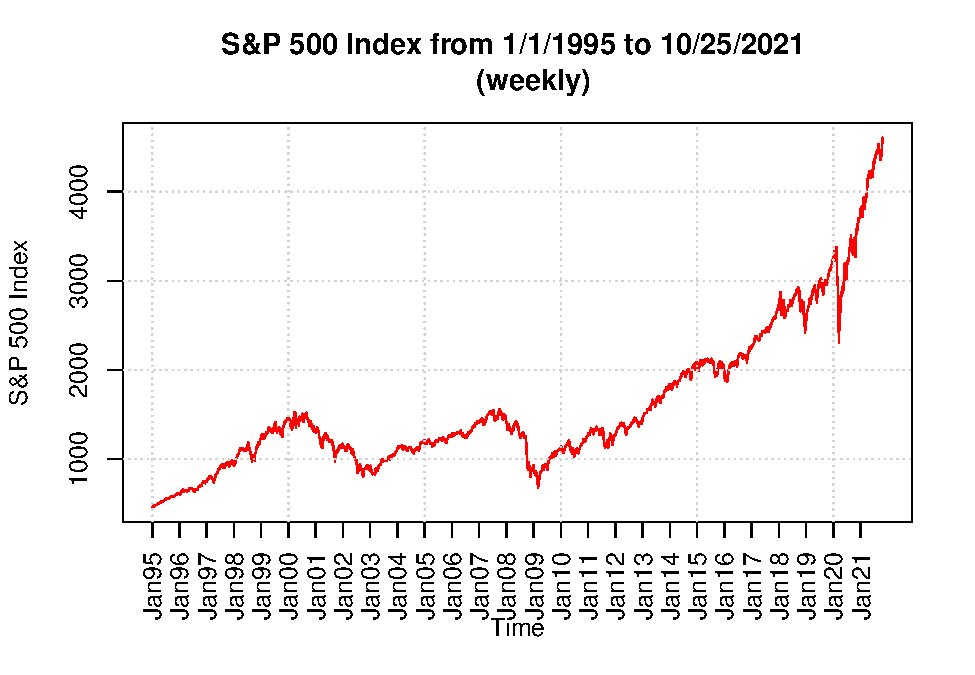
\includegraphics{02-Time-Series-Basics_files/figure-latex/unnamed-chunk-16-1.pdf}

\hypertarget{sunspots}{%
\section{Sunspots}\label{sunspots}}

Click \href{http://www.chrisbilder.com/stat878/sections/2/SN_y_tot_V2.0.csv}{SN\_y\_tot\_V2.0.csv} to download data.

\begin{Shaded}
\begin{Highlighting}[]
\NormalTok{sunspots }\OtherTok{\textless{}{-}} \FunctionTok{read.table}\NormalTok{(}\AttributeTok{file =} \StringTok{"SN\_y\_tot\_V2.0.csv"}\NormalTok{, }\AttributeTok{sep =} 
    \StringTok{";"}\NormalTok{, }\AttributeTok{col.names =} \FunctionTok{c}\NormalTok{(}\StringTok{"Mid.year"}\NormalTok{, }\StringTok{"Mean.total"}\NormalTok{, }
   \StringTok{"Mean.SD.total"}\NormalTok{, }\StringTok{"Numb.obs.used"}\NormalTok{, }\StringTok{"Definitive"}\NormalTok{))}
\end{Highlighting}
\end{Shaded}

\begin{Shaded}
\begin{Highlighting}[]
\FunctionTok{head}\NormalTok{(sunspots)}
\CommentTok{\#\textgreater{}   Mid.year Mean.total Mean.SD.total Numb.obs.used}
\CommentTok{\#\textgreater{} 1   1700.5        8.3            {-}1            {-}1}
\CommentTok{\#\textgreater{} 2   1701.5       18.3            {-}1            {-}1}
\CommentTok{\#\textgreater{} 3   1702.5       26.7            {-}1            {-}1}
\CommentTok{\#\textgreater{} 4   1703.5       38.3            {-}1            {-}1}
\CommentTok{\#\textgreater{} 5   1704.5       60.0            {-}1            {-}1}
\CommentTok{\#\textgreater{} 6   1705.5       96.7            {-}1            {-}1}
\CommentTok{\#\textgreater{}   Definitive}
\CommentTok{\#\textgreater{} 1          1}
\CommentTok{\#\textgreater{} 2          1}
\CommentTok{\#\textgreater{} 3          1}
\CommentTok{\#\textgreater{} 4          1}
\CommentTok{\#\textgreater{} 5          1}
\CommentTok{\#\textgreater{} 6          1}
\end{Highlighting}
\end{Shaded}

\begin{Shaded}
\begin{Highlighting}[]
\FunctionTok{tail}\NormalTok{(sunspots)}
\CommentTok{\#\textgreater{}     Mid.year Mean.total Mean.SD.total Numb.obs.used}
\CommentTok{\#\textgreater{} 316   2015.5       69.8           6.4          8903}
\CommentTok{\#\textgreater{} 317   2016.5       39.8           3.9          9940}
\CommentTok{\#\textgreater{} 318   2017.5       21.7           2.5         11444}
\CommentTok{\#\textgreater{} 319   2018.5        7.0           1.1         12611}
\CommentTok{\#\textgreater{} 320   2019.5        3.6           0.5         12884}
\CommentTok{\#\textgreater{} 321   2020.5        8.8           4.1         14440}
\CommentTok{\#\textgreater{}     Definitive}
\CommentTok{\#\textgreater{} 316          1}
\CommentTok{\#\textgreater{} 317          1}
\CommentTok{\#\textgreater{} 318          1}
\CommentTok{\#\textgreater{} 319          1}
\CommentTok{\#\textgreater{} 320          1}
\CommentTok{\#\textgreater{} 321          1}
\end{Highlighting}
\end{Shaded}

\begin{Shaded}
\begin{Highlighting}[]
\FunctionTok{dev.new}\NormalTok{(}\AttributeTok{width =} \DecValTok{8}\NormalTok{, }\AttributeTok{height =} \DecValTok{6}\NormalTok{, }\AttributeTok{pointsize =} \DecValTok{10}\NormalTok{)}

\CommentTok{\#again, we did not specify y{-}axis here}
\FunctionTok{plot}\NormalTok{(}\AttributeTok{x =}\NormalTok{ sunspots}\SpecialCharTok{$}\NormalTok{Mean.total, }\AttributeTok{ylab =} \StringTok{"Number of }
\StringTok{    sunspots"}\NormalTok{, }\AttributeTok{xlab =} \StringTok{"t (time)"}\NormalTok{, }\AttributeTok{type =} \StringTok{"l"}\NormalTok{, }\AttributeTok{col =} \StringTok{"red"}\NormalTok{, }
    \AttributeTok{main =} \StringTok{"Sunspots per year from 1700 to 2020"}\NormalTok{,}
    \AttributeTok{panel.first =} \FunctionTok{grid}\NormalTok{(}\AttributeTok{col =} \StringTok{"gray"}\NormalTok{, }\AttributeTok{lty =} \StringTok{"dotted"}\NormalTok{))}

\FunctionTok{points}\NormalTok{(}\AttributeTok{x =}\NormalTok{ sunspots}\SpecialCharTok{$}\NormalTok{Mean.total, }\AttributeTok{pch =} \DecValTok{20}\NormalTok{, }\AttributeTok{col =} \StringTok{"blue"}\NormalTok{)}
\end{Highlighting}
\end{Shaded}

\begin{Shaded}
\begin{Highlighting}[]
\CommentTok{\# Include dates}
\FunctionTok{plot}\NormalTok{(}\AttributeTok{y =}\NormalTok{ sunspots}\SpecialCharTok{$}\NormalTok{Mean.total, }\AttributeTok{x =}\NormalTok{ sunspots}\SpecialCharTok{$}\NormalTok{Mid.year, ylab }
    \OtherTok{=} \StringTok{"Number of sunspots"}\NormalTok{, }\AttributeTok{xlab =} \StringTok{"Year"}\NormalTok{, }\AttributeTok{type =} \StringTok{"l"}\NormalTok{, col }
    \OtherTok{=} \StringTok{"red"}\NormalTok{, }\AttributeTok{main =} \StringTok{"Sunspots per year from 1700 to 2020"}\NormalTok{,}
    \AttributeTok{panel.first =} \FunctionTok{grid}\NormalTok{(}\AttributeTok{col =} \StringTok{"gray"}\NormalTok{, }\AttributeTok{lty =} \StringTok{"dotted"}\NormalTok{))}

\FunctionTok{points}\NormalTok{(}\AttributeTok{y =}\NormalTok{ sunspots}\SpecialCharTok{$}\NormalTok{Mean.total, }\AttributeTok{x =}\NormalTok{ sunspots}\SpecialCharTok{$}\NormalTok{Mid.year, }
    \AttributeTok{pch =} \DecValTok{20}\NormalTok{, }\AttributeTok{col =} \StringTok{"blue"}\NormalTok{)}
\end{Highlighting}
\end{Shaded}

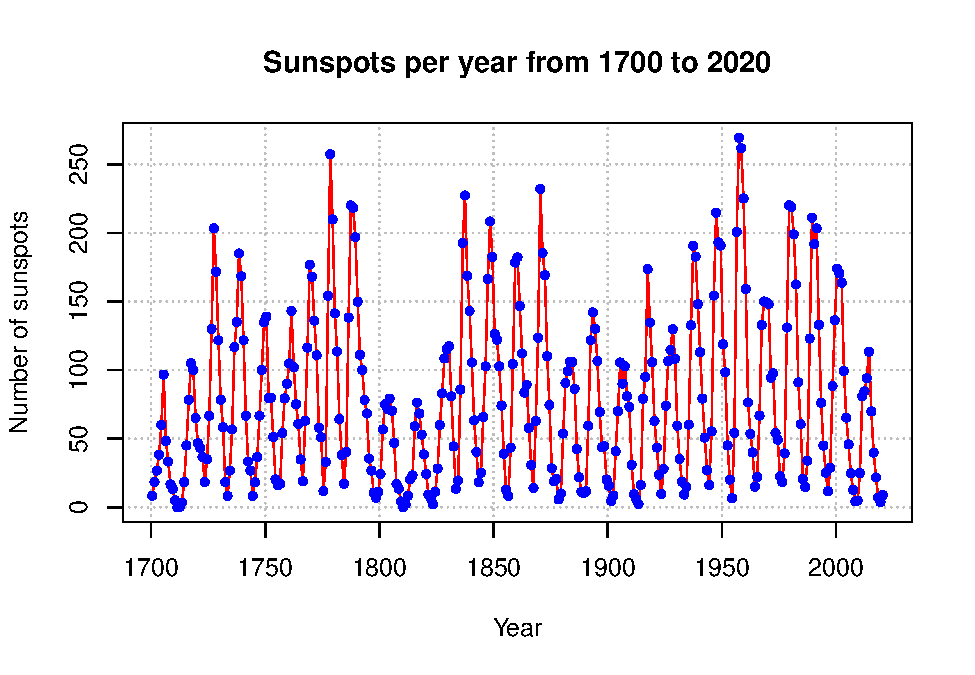
\includegraphics{02-Time-Series-Basics_files/figure-latex/unnamed-chunk-21-1.pdf}

\begin{Shaded}
\begin{Highlighting}[]
\CommentTok{\#Convert to an object of class "ts"}

\NormalTok{x }\OtherTok{\textless{}{-}} \FunctionTok{ts}\NormalTok{(}\AttributeTok{data =}\NormalTok{ sunspots}\SpecialCharTok{$}\NormalTok{Mean.total, }\AttributeTok{start =} \DecValTok{1700}\NormalTok{, frequency }
    \OtherTok{=} \DecValTok{1}\NormalTok{)}

\NormalTok{x}
\CommentTok{\#\textgreater{} Time Series:}
\CommentTok{\#\textgreater{} Start = 1700 }
\CommentTok{\#\textgreater{} End = 2020 }
\CommentTok{\#\textgreater{} Frequency = 1 }
\CommentTok{\#\textgreater{}   [1]   8.3  18.3  26.7  38.3  60.0  96.7  48.3  33.3  16.7}
\CommentTok{\#\textgreater{}  [10]  13.3   5.0   0.0   0.0   3.3  18.3  45.0  78.3 105.0}
\CommentTok{\#\textgreater{}  [19] 100.0  65.0  46.7  43.3  36.7  18.3  35.0  66.7 130.0}
\CommentTok{\#\textgreater{}  [28] 203.3 171.7 121.7  78.3  58.3  18.3   8.3  26.7  56.7}
\CommentTok{\#\textgreater{}  [37] 116.7 135.0 185.0 168.3 121.7  66.7  33.3  26.7   8.3}
\CommentTok{\#\textgreater{}  [46]  18.3  36.7  66.7 100.0 134.8 139.0  79.5  79.7  51.2}
\CommentTok{\#\textgreater{}  [55]  20.3  16.0  17.0  54.0  79.3  90.0 104.8 143.2 102.0}
\CommentTok{\#\textgreater{}  [64]  75.2  60.7  34.8  19.0  63.0 116.3 176.8 168.0 136.0}
\CommentTok{\#\textgreater{}  [73] 110.8  58.0  51.0  11.7  33.0 154.2 257.3 209.8 141.3}
\CommentTok{\#\textgreater{}  [82] 113.5  64.2  38.0  17.0  40.2 138.2 220.0 218.2 196.8}
\CommentTok{\#\textgreater{}  [91] 149.8 111.0 100.0  78.2  68.3  35.5  26.7  10.7   6.8}
\CommentTok{\#\textgreater{} [100]  11.3  24.2  56.7  75.0  71.8  79.2  70.3  46.8  16.8}
\CommentTok{\#\textgreater{} [109]  13.5   4.2   0.0   2.3   8.3  20.3  23.2  59.0  76.3}
\CommentTok{\#\textgreater{} [118]  68.3  52.9  38.5  24.2   9.2   6.3   2.2  11.4  28.2}
\CommentTok{\#\textgreater{} [127]  59.9  83.0 108.5 115.2 117.4  80.8  44.3  13.4  19.5}
\CommentTok{\#\textgreater{} [136]  85.8 192.7 227.3 168.7 143.0 105.5  63.3  40.3  18.1}
\CommentTok{\#\textgreater{} [145]  25.1  65.8 102.7 166.3 208.3 182.5 126.3 122.0 102.7}
\CommentTok{\#\textgreater{} [154]  74.1  39.0  12.7   8.2  43.4 104.4 178.3 182.2 146.6}
\CommentTok{\#\textgreater{} [163] 112.1  83.5  89.2  57.8  30.7  13.9  62.8 123.6 232.0}
\CommentTok{\#\textgreater{} [172] 185.3 169.2 110.1  74.5  28.3  18.9  20.7   5.7  10.0}
\CommentTok{\#\textgreater{} [181]  53.7  90.5  99.0 106.1 105.8  86.3  42.4  21.8  11.2}
\CommentTok{\#\textgreater{} [190]  10.4  11.8  59.5 121.7 142.0 130.0 106.6  69.4  43.8}
\CommentTok{\#\textgreater{} [199]  44.4  20.2  15.7   4.6   8.5  40.8  70.1 105.5  90.1}
\CommentTok{\#\textgreater{} [208] 102.8  80.9  73.2  30.9   9.5   6.0   2.4  16.1  79.0}
\CommentTok{\#\textgreater{} [217]  95.0 173.6 134.6 105.7  62.7  43.5  23.7   9.7  27.9}
\CommentTok{\#\textgreater{} [226]  74.0 106.5 114.7 129.7 108.2  59.4  35.1  18.6   9.2}
\CommentTok{\#\textgreater{} [235]  14.6  60.2 132.8 190.6 182.6 148.0 113.0  79.2  50.8}
\CommentTok{\#\textgreater{} [244]  27.1  16.1  55.3 154.3 214.7 193.0 190.7 118.9  98.3}
\CommentTok{\#\textgreater{} [253]  45.0  20.1   6.6  54.2 200.7 269.3 261.7 225.1 159.0}
\CommentTok{\#\textgreater{} [262]  76.4  53.4  39.9  15.0  22.0  66.8 132.9 150.0 149.4}
\CommentTok{\#\textgreater{} [271] 148.0  94.4  97.6  54.1  49.2  22.5  18.4  39.3 131.0}
\CommentTok{\#\textgreater{} [280] 220.1 218.9 198.9 162.4  91.0  60.5  20.6  14.8  33.9}
\CommentTok{\#\textgreater{} [289] 123.0 211.1 191.8 203.3 133.0  76.1  44.9  25.1  11.6}
\CommentTok{\#\textgreater{} [298]  28.9  88.3 136.3 173.9 170.4 163.6  99.3  65.3  45.8}
\CommentTok{\#\textgreater{} [307]  24.7  12.6   4.2   4.8  24.9  80.8  84.5  94.0 113.3}
\CommentTok{\#\textgreater{} [316]  69.8  39.8  21.7   7.0   3.6   8.8}
\end{Highlighting}
\end{Shaded}

\begin{Shaded}
\begin{Highlighting}[]
\FunctionTok{class}\NormalTok{(x)}
\CommentTok{\#\textgreater{} [1] "ts"}

\FunctionTok{class}\NormalTok{(sunspots}\SpecialCharTok{$}\NormalTok{Mean.total)}
\CommentTok{\#\textgreater{} [1] "numeric"}
\end{Highlighting}
\end{Shaded}

\hypertarget{plot.ts}{%
\subsection{plot.ts()}\label{plot.ts}}

plot() is a generic function - uses the plot.ts() method function

\begin{Shaded}
\begin{Highlighting}[]
\CommentTok{\# we did not specify y{-}axis here, but x is now ts}
\FunctionTok{plot}\NormalTok{(}\AttributeTok{x =}\NormalTok{ x, }\AttributeTok{ylab =} \FunctionTok{expression}\NormalTok{(}\FunctionTok{paste}\NormalTok{(x[t], }\StringTok{" (Number of }
\StringTok{   sunspots)"}\NormalTok{)), }\AttributeTok{xlab =} \StringTok{"Year"}\NormalTok{, }\AttributeTok{type =} \StringTok{"o"}\NormalTok{, }\AttributeTok{col =} \StringTok{"red"}\NormalTok{, main }
   \OtherTok{=} \StringTok{"Sunspots per year from 1700 to 2020"}\NormalTok{)}
\CommentTok{\#\textgreater{} Warning in title(main = main, xlab = xlab, ylab = ylab,}
\CommentTok{\#\textgreater{} ...): font metrics unknown for character 0xa}

\CommentTok{\#\textgreater{} Warning in title(main = main, xlab = xlab, ylab = ylab,}
\CommentTok{\#\textgreater{} ...): font metrics unknown for character 0xa}
\end{Highlighting}
\end{Shaded}

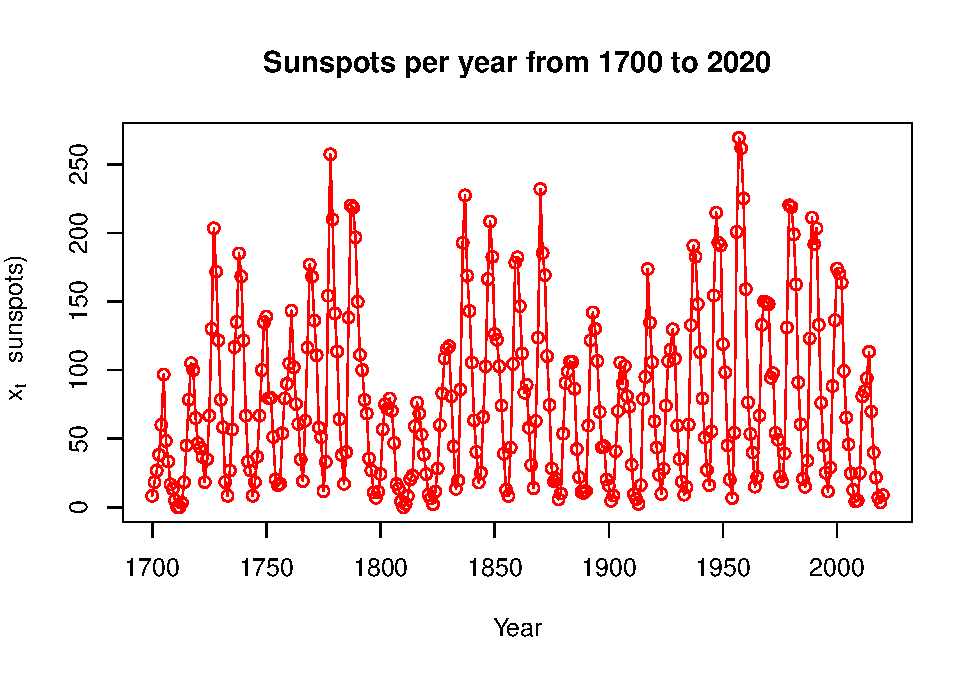
\includegraphics{02-Time-Series-Basics_files/figure-latex/unnamed-chunk-24-1.pdf}

  \bibliography{book.bib,packages.bib}

\end{document}
